


\chapter{Generalidades y ecuaciones de primer orden}

\section{¿Que son las ecuaciones diferenciales?}


\begin{definicion}[Ecuación diferencial, definición informal]{}
 Es una o varias relaciones entre una o varias variables dependientes y sus tasas de cambio respecto a ciertas variables independientes.
 \end{definicion}

 El problema básico asociado
 a las ecuaciones diferenciales es hallar las variables dependientes que las resuelven.

 Las ecuaciones diferenciales son usadas muy a menudo en matemática aplicada, puesto que muchas
 leyes (de la física por ejemplo) se expresan atraves de este tipo de ecuaciones.








 \begin{ejemplo}[\href{http://es.wikipedia.org/wiki/Caída_libre}{Caída libre}]{} Modelizar matemáticamente el movimiento de un cuerpo de masa $m$ en las proximidades de la superficie
terrestre, asumiendo que su movimiento es
sobre la vertical y que las fuerzas que sobre él actúan son la gravedad y el rozamiento con el aire.
\end{ejemplo}

\begin{wrapfigure}[20]{l}{6cm}
  \begin{center}
  \setlength{\unitlength}{1cm}
    \begin{picture}(5, 5)(0,1)
      \put(1,2){\vector(0,1){3.5}}
      \put(1,2){\vector(0,-1){1}}
      \put(0,2){\vector(1,0){5}}
      \multiput(0,2)(.25,0){20}{\line(-1,-1){0.5}}
      \put(2,4){\circle*{.5}}
      \put(2,4){\vector(0,-1){1.5}}
      \put(2.3,3){$F_{\hbox{grav}}=mg\approx 9.8 m/s^2$}
      \put(2,4){\vector(0,1){1.5}}
      \put(2.3,5){$F_{\hbox{roz}}=-cv$}
      \multiput(1,4)(.1,0){10}{\line(1,0){0.05}}
      \put(0,4){$x(t)$}
      \put(0,1){$x>0$}
      \put(0,5){$x<0$}

    \end{picture}\caption{Caída libre}\label{fig:caída}
  \end{center}
\end{wrapfigure}
\noindent $x(t)=$ posición a lo largo de la vertical, relativo a un eje de coordenadas\newline
$v(t)=\frac{dx}{dt}=$ velocidad\newline
$F_{grav}=$ fuerza debida a la gravedad $=mg$ donde $g=9.8m/s^2$
$F_{roz}=$ fuerza de rozamiento, proporcional a la velocidad y de sentido
contrario $=-cv$, $c>0$.




 Usamos la \href{http://es.wikipedia.org/wiki/Leyes_de_Newton}{Segunda Ley de Newton}, esto es la suma de las fuerzas totales que actuan sobre un cuerpo de masa $m$
es igual al producto de la masa $m$ y la aceleración $a(t)$.
Recordemos que la aceleración es la tasa de cambio de la velocidad, es decir la derivada 
segunda de la posición.   

  Usando todas las relaciones mencionadas

\[\begin{split} ma(t)&=mv'(t)=F_{\hbox{total}}\\
  &=F_{\hbox{grav}}+F_{\hbox{roz}}\\
  &=mg-cv
\end{split}
\]
vale decir
\begin{equation}\label{caidaLibre1}
 \boxed{ x''(t)+\frac{c}{m} x'(t)=g.}
\end{equation}
\begin{equation}\label{caidaLibre2}
\boxed{ v'(t)+\frac{c}{m} v=g.}
\end{equation}





\section{Algunos conceptos relacionados con ecuaciones diferenciales}

\begin{definicion}[Orden]{} El índice de la mayor derivada interviniente en la ecuación.
 \end{definicion}

 Por ejemplo la ecuación \eqref{caidaLibre1} es de orden 2 y la
ecuación \eqref{caidaLibre2}, si bien está estrechamente relacionada con la anterior, es de orden 1. Como regla casi general, cuanto menor es el orden,  más fáciles de estudiar y/o resolver las ecuaciones son.

  \begin{definicion}[Solución]{} Una función que satisface la relación que indica la ecuación.

   \end{definicion}

   Por ejemplo
\begin{equation}\label{SolGencaidaLibre2} v(t)=\frac{m}{c}g+ke^{-\frac{c}{m}t},\end{equation}
resuelve \eqref{caidaLibre2}, para todo $C\in\rr$. No deberíamos perder tiempo en chequear una cuestión tan sencilla, pero aprovechemos la ocasión para usar  \href{http://www.sympy.org}{SymPy}.





 \begin{pyverbatim}
>>>from sympy import *
>>>m,g,c,k,t=symbols('m,g,c,k,t')
>>>v=m/c*g+k*exp(-c/m*t)
>>>simplify(v.diff(t)+c/m*v)
g
 \end{pyverbatim}
Notar que las líneas que comienzan con el signo del prompt \verb~>>>~ indican entradas por línea de comandos y las que comienzan sin este signo son las respuestas del interprete.

Rara vez utilizaremos las siguientes funcionalidades de sympy, pero es oportuno decir que
 \texttt{SymPy} puede encontrar la solución a una ecuación diferencial

 \begin{pyverbatim}
>>>v=symbols('v',cls=Function)
>>>EqCaida=Eq(v(t).diff(t)+c/m*v(t),g)
>>>Vel=dsolve(EqCaida,v(t))
>>> Vel
v(t) == (g*m + exp(c*(C1 - t/m)))/c
 \end{pyverbatim}

La solución obtenida es la ya conocida. Es instructivo averiguar que tipo de dato tiene la variable \verb~Vel~

 \begin{pyverbatim}
>>> type(Vel)
<class 'sympy.core.relational.Equality'>
 \end{pyverbatim}
A este tipo de cuestiones hay que prestar atención cuando se trabaja con sympy, 
pues existe la tendencia a confudir los conceptos matemáticos con los propios del lenguaje. 
Por ejemplo, matemáticamente una solución es una función. Sin embargo, en este caso, 
cuando le solicitamos una solución a sympy nos entrega un objeto de tipo  
``relación de igualdad''.





\begin{definicion}[Ecuación diferencial ordinaria (EDO)]{} Es una ecuación donde las variables dependientes sólo dependen de una única variable independiente.
\end{definicion}

Las
ecuaciones \eqref{caidaLibre1} y \eqref{caidaLibre2} son ejemplo de ello, la variable independiente es el tiempo.
  \begin{definicion}[Ecuación en derivadas parciales (EDP)]{} Es una ecuación donde las variables dependientes dependen de más de una variable independiente.
   \end{definicion}

Ejemplo de este tipo de ecuación es la ecuación de Laplace

\[\frac{\partial^2 u}{\partial x^2}+\frac{\partial^2 u}{\partial y^2}=0\]

Puede ocurrir también que dispongamos de varias ecuaciones diferenciales
que se deben satisfacer simultaneamente. 
En estos casos, el conjuntos de ecuaciones se suele escribir como una única 
ecuación vectorial. Por este motivo, en algunas ocasiones cuando dispongamos de una
única ecuación diremos que tenemos una \emph{ecuación  escalar}.

\begin{definicion}[Sistema de ecuaciones]{} Es un  conjunto de ecuaciones diferenciales que se deben satisfacer simultaneamente.
 \end{definicion}

En ese caso es  de esperar que tengamos varias incognitas en
nuestro problema. En general una ecuación escalar determina sólo una incognita. De hecho aquí ocurre, a semejanza con ecuaciones algebraicas, que es frecuente necesitar tantas ecuaciones como incognitas.

\begin{ejemplo}[Ecuación del péndulo]{} El sistema de ecuaciones:
\[\left\{ \begin{array}{l l} x'&=y \\y'&=-\sen(x) \end{array}\right.\]
es muy conocido pues modeliza el movimiento de un péndulo.
\end{ejemplo}



Muy a menudo hablaremos de resolver una ecuación, pero es oportuno discutir que queremos significar con esto.

\begin{definicion}[Resolver una ecuación]{} Es expresar la solución como combinaciones algebraicas y composiciones de funciones que consideramos elementales.
\end{definicion}

Esta definición contiene una vaga apelación a ciertas ``funciones elementales''. El universo de funciones que se considera elemental es una cuestión política, no matemática. En  principio, consideraremos elementales a las potencias, exponenciales, logarítmos, trigonométricas y trigonométricas inversas. No obstante esta lista se puede expandir con muchas funciones especiales.  Las operaciones permitidas para combinar estas funciones
también están sujetas a convenciones. Por ejemplo, admitiremos como válida una expresión que contenga una integral, al menos en el caso que no sea claro como resolver esta integral.

 Casi todo este curso trata con la discusión de métodos para resolver ecuaciones.  
 Sin embargo resolver ecuaciones no es quizás el problema principal relacionado 
 con las ecuaciones diferenciales. No importa tanto lograr una expresión 
 formal de la solución, como, por ejemplo, conocer las propiedades que poseen las soluciones. 
 Al fin y al cabo, uno conoce una función a través de sus propiedades.
 





\begin{definicion}[Solución general]{} Usualmente una ecuación presenta infinitas soluciones. Una solución general  es una expresión que representa todas estas soluciones. Es habitual que una solución general contenga parámetros. Cada elección de estos parámetros determina una solución distinta.
 \end{definicion}

 Por ejemplo \eqref{SolGencaidaLibre2} es la solución general de \eqref{caidaLibre2}.
  La afirmación anterior requiere una demostración puesto que sólo hemos mostrado que \eqref{SolGencaidaLibre2} es solución, pero no
que toda solución se expresa con \eqref{SolGencaidaLibre2}. Para demostrar la afirmación, hay que multiplicar ambos miembros de \eqref{caidaLibre2} 
por $e^{\frac{c}{m}t}$ y luego integrar respecto a $t$ 
\[\frac{mg}{c}e^{\frac{c}{m}t}=\int ge^{\frac{c}{m}t}dt=\int v'(t)e^{\frac{c}{m}t}+\frac{c}{m}e^{\frac{c}{m}t} vdt=e^{\frac{c}{m}t}v+C.\]
 Despejando $v$ del primer y último miembro obtenemos \eqref{SolGencaidaLibre2} con $k=-C$.

 




\begin{ejemplo}{} En algunas ocasiones sólo podemos dejar una relación implícita entre las variable dependientes e independientes. Por ejemplo
\begin{equation}\label{solImpl}x=e^y+y+C\quad\text{ para } C\in\rr\end{equation}
es solución general de
\[y'(e^y+1)=1.\]
Vamos a chequear sólo que \eqref{solImpl} es solución, dejando la justificación que toda solución tiene esa forma para más adelante. Derivando \eqref{solImpl}
\[ 1=e^yy'+y'\]
Luego $y'=1/(1+e^{y})$. Reemplazando esta relación  en la ecuación diferencial corroboramos que es solución.
\end{ejemplo}



\section{Definición formal}

\begin{definicion}[Ecuación diferencial]{def:eq} Una ecuación diferencial
ordinaria de orden $n$ es una relación de la forma
\[\boxed{F(x,y(x),y'(x),\ldots,y^{(n)}(x))=0}.\]
donde $F:(a,b)\times \Omega\to\rr$, $\Omega$ es abierto de $\rr^{n+1}$ y $(a,b)$ un intervalo de $\rr$.
  \end{definicion}





\begin{ejemplo}{} El problema de hallar una primitiva de una función es una ecuación
diferencial que, como ya se ha visto en cursos iniciales de análisis, se relaciona con el concepto de integral. Supongamos $f:(a,b)\subset \rr\to\rr$ una función continua. Consideremos la ecuación diferencial
\[y'(x)=f(x).\]
Sea $x_0\in(a,b)$, integrando respecto a $x$ entre $x_0$ y $x$
\[y(x)=y(x_0)+\int_{x_0}^xf(t)dt\]
Que es una solución general. Quedaría determinada una única solución si, por ejemplo, conociecemos $y(x_0)$.
\end{ejemplo}



\begin{ejemplo}{} Supongamos $f:(a,b)\subset \rr\to\rr$ como antes. Consideremos la ecuación diferencial
\[y''(x)=f(x).\]
Tomemos una integral indefinida respecto a $x$ 
\[y'(x)=C_1+\int f(t)dt\]
Ahora deberemos tomar una integral indefinida más
\[y(x)=C_2+C_1t +\int\left(\int f(x)dx\right)dx.\]
Ahora quedan dos constantes $C_1$ y $C_2$. 
\end{ejemplo}

En el caso de un sistema de ecuaciones diferenciales, la forma de describirlo es esencialmente 
 igual a la de la Definición \ref{def:eq}. La nueva definición contiene a la Definición \ref{def:eq}
 como caso particular.

 \begin{definicion}[Sistema de ecuación diferenciales]{def:sist_eq} 
 Una sistema de $k$-ecuaciones diferenciales ordinarias de orden $n$ 
 es una relación de la forma
\[\boxed{F(x,y(x),y'(x),\ldots,y^{(n)}(x))=0}.\]
donde $F:(a,b)\times \Omega\to\rr^k$, 
\[\Omega\subset\underbrace{\rr^k\times\cdots\times\rr^k}_{n+1-\hbox{veces}}\]
es abierto y $(a,b)$ un intervalo de $\rr$. Notar que el $=$ en la derecha de la ecuación está
en $\rr^k$ y que tenemos $k$ ecuaciones e incognitas, las $k$ componentes de
$y=(y_1,\ldots y_k)$.
  \end{definicion}
  
\begin{ejemplo}{}
 En el caso del péndulo  $k=2$, $n=1$, mientras que $(a,b)=\rr$, $\Omega=\rr\times\rr$ y
 $F:\rr^2\times \rr^2\to\rr^2$ viene dada por
 \[F\left(\begin{pmatrix}
      x \\ v
     \end{pmatrix}
,\begin{pmatrix}
  \xi \\ \eta 
  \end{pmatrix}
  \right)
  =\begin{pmatrix} \xi-v \\ \eta+\sen(x)  \end{pmatrix}
\]
\end{ejemplo}
Más adelante veremos que toda ecuación, o sistemas de ecuaciones, ordinaria de orden $n$ 
se puede reducir a un sistema de orden $1$. De modo tal que es más frecuente considerar
este tipo de sistemas. También es común considerar, se trate ya de ecuaciones 
escalares o sistemas,
 ecuaciones donde es posible despejar 
de manera explícita la derivada de mayor orden. A esta forma la denominaremos 
\emph{forma explícita} de la ecuación

\boxedeq{ y^{(n)}(x)=f(x,y(x),y'(x),\ldots,y^{(n-1)}(x)).}{eq:eq_expl}


\section{Problemas bien planteados, condiciones iniciales}

La siguiente definición expresa lo que entenderemos cuando digamos que un problema está bien planteado.


 \begin{definicion}[Principio de Hadamard]{defi:had}
 Un problema se dice  \href{http://es.wikipedia.org/wiki/Problema_bien_definido}{bien planteado} segun Hadamard si satisface que

 \begin{enumerate}
  \item\label{it:had1} El problema admite solución
  \item\label{it:had2} La solución es única
  \item\label{it:had3} La solución depende de manera continua de los datos numéricos del problema.
 \end{enumerate}
\end{definicion}
 \marginpar{
    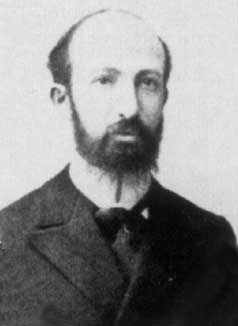
\includegraphics[scale=.3]{imagenes/hadamard.jpg}\\
    Jacques Hadamard (1865-1963)
}
 Como hemos visto, una ecuación diferencial no determina una única solución, por consiguiente no sería un problema bien planteado. Debemos agregar relaciones
a nuestro problema para que sea bien planteado. Es así que aparecen condiciones iniciales, problemas de contorno, etc.




\begin{definicion}[Problemas de valores iniciales (PVI)]{} Sea $x_0\in(a,b)$, $F:(a,b)\times \Omega\to\rr$ e $y_0,y_0^1,\ldots,y_0^{n-1}\in\rr$. Las siguientes relaciones  se denominan problema de
valores iniciales
\begin{equation}\label{eq:pvi}
 \left\{\begin{array}{l l l}
         F(x,y,y',&\ldots,y^{(n)})=0& x\in(a,b)\\
         y(x_0)&=y_0&\\
         y'(x_0)&=y_0^1&\\
          & \vdots &\\
          y^{(n-1)}(x_0)&=y_0^{n-1}&\\
        \end{array}
   \right.
\end{equation}

\end{definicion}

Más delante demostraremos el teorema de existencia y unicidad para ecuaciones y sistemas de ecuaciones. Este teorema nos dice que, para ciertas $F$, el problema \eqref{eq:pvi} tiene una única solución alrededor de un entorno de $x_0$.

Es común en las aplicaciones físicas de las EDO, que la variable $x$ represente el tiempo e $y=y(x)$ represente alguna cantidad física (posición, velocidad, temperatura, etc) caracterizando a cierto sistema físico. Es muy frecuente que aparezcan ecuaciones de orden $2$  ($n=2$). En esta situación, al par $(y,y')$ se lo denomina \emph{estado} del sistema y las condiciones \ref{it:had1} y \ref{it:had2} en la Definición \ref{defi:had} se leen como que el estado del sistema en un momento $x_0$ dado determina el estado del mismo en cualquier otro momento. Este es el postulado principal de la corriente  filosófica conocida por   \href{https://es.wikipedia.org/wiki/Determinismo}{determinismo} .

 Es común que una ecuación que modela un sistema físico dependa de parámetros. Pensar por ejemplo del papel de la masa en la ecuación \eqref{caidaLibre1}. Estos parámetros o incluso los valores iniciales del problema \eqref{eq:pvi} dependen muchas veces de resultados de mediciones y sólo es posible tener de ellos un valor aproximado. Por consiguiente,casi nunca se resuelve el PVI que se debería resolver, sino otro, con parámetros y valores iniciales aproximadamente iguales a los correctos\footnote{Estamos usando una noción bastante ingenua de corrección}.
 La condición \ref{it:had3} en la Definición \ref{defi:had} expresa el hecho de que la soluciones a PVIs aproximadamente iguales son aproximadamente iguales entre si.


 Vamos a destacar la siguiente instancia particular de la Definición \ref{eq:pvi}.


\begin{definicion}[PVI para ecuaciones de primer orden]{} La ecuación general de primer orden tiene la forma
\[
F(x,y(x),y'(x))=0,
\]
donde $F:(a,b)\times \Omega\to\rr$ y $\Omega$ abierto de $\rr^2$. Con frecuencia asumiremos que $y'$ se despeja de la relación anterior, es decir que existe $f:\Omega'\to\rr$,
$\Omega'$ abierto de $\rr^2$, tal que
\[y'=f(x,y).\]
Bajo esta suposición, si $(x_0,y_0)\in\Omega'$ el problema de valores iniciales se escribe
\[\left\{\begin{array}{l l}
	    y'&=f(x,y)\\
	    y(x_0)&=y_0
         \end{array}\right.
\]
\end{definicion}



\section{Familias paramétricas de funciones}

Hemos dicho que en el común de los casos es de esperar que una
ecuación tenga asociado un conjunto de soluciones. En esta sección vamos a preguntarnos sobre el problema inverso, dao un conjunto de funciones encontrar una ecuación que lo tenga por solución.



\begin{mdframed}[style=MiEstilo]\relax%
\textbf{Problema. }
Dada una familia paramétrica de funciones
 \begin{equation}\label{flia_param}y=y(x,c),\end{equation}
 dependiente del parámetro $c\in\rr$, ¿Será posible hallar una ecuación para la cual la familia sea la solución general?
\end{mdframed}

En líneas generales la respuesta es si. Nos conviene expresar \eqref{flia_param} como una ecuación implícita
\begin{equation}\label{flia_impl}f(x,y,c)=0.\end{equation}
Derivando esta ecuación respecto a $x$
\begin{equation}\label{der_impl}
 \frac{\partial f}{\partial x}+\frac{\partial f}{\partial y}y'(x,c)=0.
\end{equation}
Ahora es posible eliminar $c$ de \eqref{flia_impl} y \eqref{der_impl} al costo de quedarnos con una sola ecuación.




\begin{ejemplo}{} Encontrar la ecuación que satisface la familia paramétrica
\[x^2+y^2=c^2.\]
Derivamos
\[2x+2yy'=0.\]
Ya está!!!
\end{ejemplo}

\begin{ejemplo}{} Idem $x^2+y^2=2cx$.  Derivando
\[2x+2yy'=2c.\]
Eliminamos $c$ de las dos relaciones
\[\frac{x^2+y^2}{x}=2x+2yy'\Rightarrow \boxed{y'=\frac{y^2-x^2}{2xy}}.\]
\end{ejemplo}

\begin{mdframed}[style=MiEstilo]\relax%
 Dada una familia paramétrica
 \[f(x,y,c)=0,\]
 encontrar otra
 \[g(x,y,d)=0\]
 tal que los ángulos que forman los gráficos entre las funciones de una y de otra familia sean rectos  en cada punto de corte entre ellos.
\end{mdframed}




Para resolver este problema se completan estos pasos
\begin{itemize}
 \item Se encuentra la ecuación diferencial que satisface la familia dada, digamos
 \[y'=h(x,y).\]
 \item Se resuelve
 \[y'=-\frac{1}{h(x,y)}.\]
\end{itemize}




\begin{ejemplo}{} Encontrar la familia de curvas ortogonales a la flia de circunferencias

\[x^2+y^2=c^2\]

Hallamos antes que la ecuación que satisfacen estas curvas es
\[y'=-\frac{x}{y}.\]
Luego deberíamos resolver
\[y'=\frac{y}{x}.\]
Que aún no sabemos resolver,  pero SymPy si!!!

\end{ejemplo}


\begin{mdframed}[style=MiEstilo]\relax%
\textbf{\texttt{dsolve}}

\textbf{Sintaxis} (ampliar en la \href{http://docs.sympy.org/latest/modules/solvers/ode.html#}{documentación \texttt{SymPy}})

\texttt{dsolve(eq, f(x), hint)}

\texttt{eq:} Ecuación (posicional)

\texttt{f(x):} función incognita (posicional)

\texttt{hint: } Método a emplear. Argumento con nombre \texttt{hint='cadena'}.

\end{mdframed}




\begin{pyverbatim}
x=symbols('x')
y=Function('y')(x)
MiEcua=Eq(y.diff(x),y/x)
f=dsolve(MiEcua,y)
\end{pyverbatim}

\noindent\textbf{Resultado:}
Flía rectas  por el origen. \\
La instrucción\\
\texttt{f=dsolve(MiEcua,y,hint='separable')}
\\produce el mismo resultado.





\begin{mdframed}[style=MiEstilo]\relax%
\textbf{\texttt{plot}}

\textbf{Sintaxis} (Ampliar en la \href{http://docs.sympy.org/latest/modules/plotting.html}{documentación \texttt{SymPy}})

Para un gráfico simple

\texttt{plot(expr,rango,opcionales(claves))}

\texttt{expr:} Expresión a graficar 

\texttt{rango:} Conjunto donde varia la variable independiente 

\texttt{opcionales } Argumentos que modifican la apariencia del gráfico. Generalemente de la forma de clave=valor

 
\end{mdframed}

\begin{ejemplo}{}

\end{ejemplo}


\begin{pyverbatim}
x=symbols('x')
f=plot(1/x,(x,-3,3),ylim=(-3,3))
\end{pyverbatim}

\noindent\textbf{Resultado:}
\begin{center}
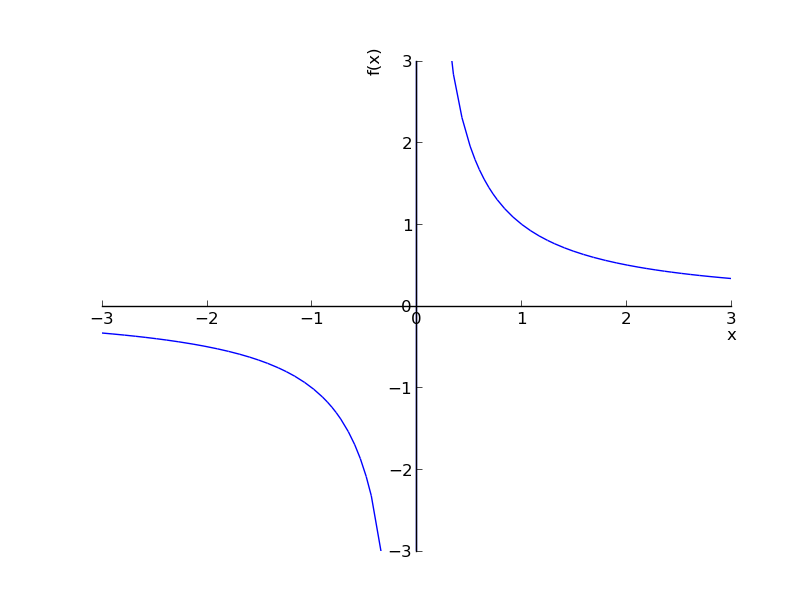
\includegraphics[scale=.35]{imagenes/ejemplo_plot.png}
\end{center}












\begin{ejemplo}{}Grafiquemos un familias paramétrica de funciones.

\end{ejemplo}



\begin{pyverbatim}
from sympy import *
x,y=symbols('x,y')
Rango=range(21)
L=[tan(pi*k/21.0) for k in Rango] 
p=plot(L[0]*x,(x,-2,2),show=False,xlim=(-2,2),\
ylim=(-2,2),aspect_ratio=(1,1))
for pend in L[1:]:
    p1=plot(pend*x,(x,-2,2),show=False,\
xlim=(-2,2),ylim=(-2,2),aspect_ratio=(1,1))
    p.append(p1[0])
for r in range(1,10):
    p1=plot_implicit(Eq(x**2 + y**2, 0.2*r),\
show=False,aspect_ratio=(1,1),xlim=(-2,2),ylim=(-2,2))
    p.append(p1[0])
p.show()
\end{pyverbatim}


\noindent\textbf{Resultado:}
\begin{figure}[h]
\begin{center}
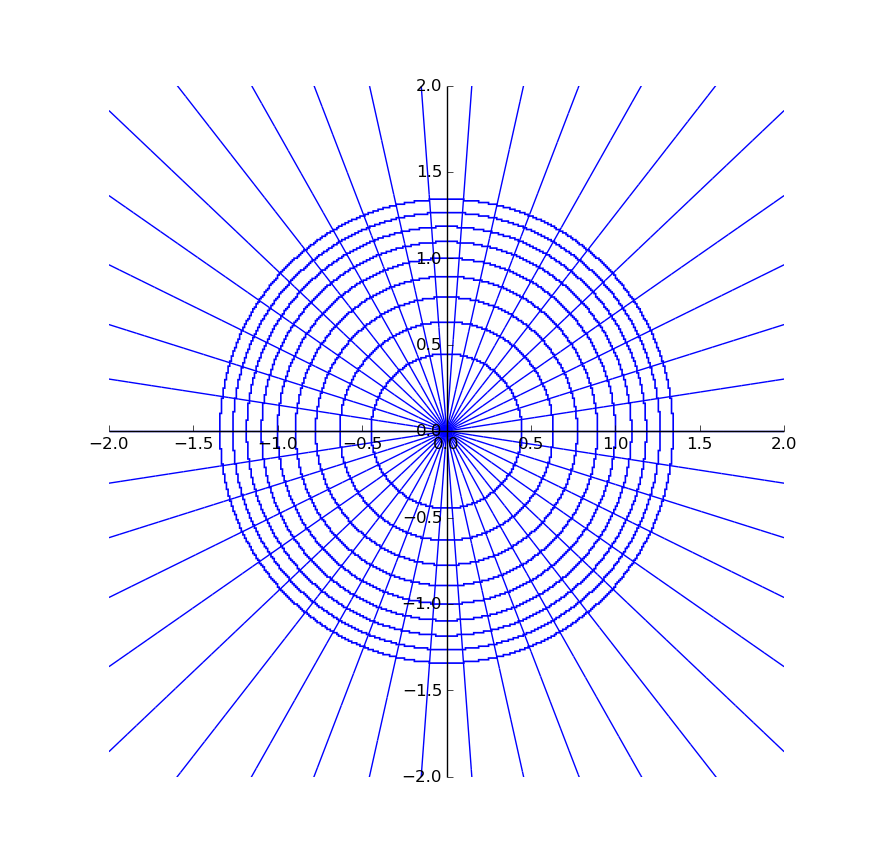
\includegraphics[scale=.2]{imagenes/flia_curvas_ortogonales.png}
\end{center}
\caption{Familia curvas ortogonales}\label{fig:ortogonales}
\end{figure}


\begin{mdframed}[style=MiEstilo]\relax% 
\textbf{Familias paramétricas de funciones en coordenadas polares.}
En ocasiones la ecuación de la familia de curvas esta dada en otras coordenadas. Por ejemplo supongamos que tenemos la flia de curvas dadas por una EDO en coordenadas polares
\[\frac{dr}{d\theta}=f(r,\theta)\label{eq:flia_curvas_polar},\]
y queremos hallar su flia ortogonal.
 
\end{mdframed}


\noindent\textbf{Solución:} Calculemos $dy/dx$ para las curvas en la familia dada.
\[\frac{dy}{dx}=\frac{dy/d\theta}{dx/d\theta}=\frac{r_{\theta}\sen\theta+r\cos\theta}{r_{\theta}\cos\theta-r\sen\theta}=\frac{f\sen\theta+r\cos\theta}{f\cos\theta-r\sen\theta},\]

donde $r_{\theta}=dr/d\theta$. La flia ortogonal tiene que satisfacer

\[\frac{dy}{dx}=-\frac{f\cos\theta-r\sen\theta}{f\sen\theta+r\cos\theta}\]
Luego
\[\frac{r_{\theta}\sen\theta+r\cos\theta}{r_{\theta}\cos\theta-r\sen\theta}=-\frac{f\cos\theta-r\sen\theta}{f\sen\theta+r\cos\theta}.\]
Si despejamos $r_{\theta}$ llegamos a la ecuación de la flia de curvas ortogonales en coordenadas polares

\boxedeq{\frac{dr}{d\theta}=-\frac{r^2}{f}.}{eq_flia_ortogonal_polares}


Aconsejamos ampliar este tema de \cite{simmons_esp}.  



\section{Separación de variables}
En esta unidad presentaremos algunos métodos de solución para ecuaciones de primer orden. Empezaremos con el, quizás, más popular de todos, el método de \emph{separación de variables}.

\begin{definicion}[Ecuaciones en variables separadas]{} Se dice que en una ecuación de primer orden
 \[y'=f(x,y)\]
 separan las variables, si es posible la factorización $f(x,y)=g(x)h(y)$.
\end{definicion}



Una ecuación  en la que se separan variables se puede resolver siguiendo los siguientes pasos. Hallamos los valores $y_0$ tales que cuando $h(y_0)=0$. Notar que para cualquiera de esos valores la función constante $y(x)\equiv y_0$  es solución. De esta manera podemos encontrar algunas soluciones por esta consideración. 

Para hallar otras, asumamos $h(y)\neq 0$. 
\[\frac{y'}{h(y)}=g(x),\]
Si $H$ y $G$ son primitivas de $1/h$ y $g$ respectivamente por la regla de la cadena tenemos
\[\frac{d}{dx}H(y)=\frac{d}{dx}G(x)\]
Luego 
\[H(y)=G(x)+C,\quad C\in\rr.\]
Por último, si podemos encontrar la inversa de $H$

\boxedeq{ y(x)=H^{-1}\left(G(x)+C\right). }{eq:var_sep}
 
será candidata a solución general. No podemos estar seguros de esta afirmación, sobre todo porque la deducción de esta fórmula estuvo sujeta a suposiciones, como $h(y)\neq 0$.



\begin{ejemplo}{} Resolver
\[y'=\frac{y}{x}.\]
Como queremos agrupar todos los factores que contienen la variable $y$ en uno de los miembros, debemos ``pasar dividiendo'' $y$. Esto es imposible si $y=0$. Reemplazando $y\equiv 0$ en la ecuación vemos que la resuelve. Así hemos encontrado nuestra primera solución $y\equiv 0$. El resto del método, es común llevarlo adelante de la siguiente forma
\[\begin{split}
   \frac{dy}{dx}=\frac{y}{x} &\Longrightarrow \frac{dy}{y}=\frac{dx}{x} \Longrightarrow \int \frac{dy}{y}=\int \frac{dx}{x}\\
   &\Longrightarrow\ln|y|=\ln|x|+C \Longrightarrow |y|= k|x|, \hbox{ con }k>0\\
   &\Longrightarrow y= kx, \hbox{ con }k\neq 0
  \end{split}
\]
\end{ejemplo}
Notar que, al fin y al cabo, la solución general es $y=kx$ con $k\in\rr$. La solución ``díscola'' $y\equiv 0$ también se escribe $y=kx$, cuando $k=0$.


\begin{mdframed}[style=MiEstilo]\relax%
\textbf{\texttt{classify\_ode}}: clasificación de ecuaciones
\textbf{Sintaxis}\\
\texttt{classify\_ode(eq, f(x))}\\
\end{mdframed}


Sympy contiene un comando que nos dice que metodo es posible aplicar a una ecuaqción dada.
\begin{pyverbatim}
x=symbols('x')
y=Function('y')(x)
MiEcua=Eq(y.diff(x),y/x)
tipo=classify_ode(MiEcua,y)
\end{pyverbatim}

\textbf{Resultado:}\\
\begin{verbatim}
('separable', '1st_exact', '1st_linear', 
'almost_linear', 'lie_group',  etc)
\end{verbatim}


\section{Aplicaciones}

Vamos a describir algunos ejemplos. Algunos de ellos llevan a problemas matemáticos muy simples. No obstante es oportuno discutirlos por dos motivos, habituarnos a la utilización de la matemática para resolver problemas de otras ciencias y sentar las bases para discutir problemas más relevantes desde una óptica matemática.

\subsection{Ley de reproducción normal}
  En muchos ejemplos de biología, química-física, etc, hay magnitudes que crecen(decrecen) siguiendo una ley que denominaremos
\href{http://es.wikipedia.org/wiki/Crecimiento_exponencial}{Ley de reproducción  normal}. Según esta ley la cantidad de individuos, sustancia, materia,
energía, etc, que se agrega o elimina de una población, cuerpo, etc por unidad de tiempo es proporcional a la cantidad de individuos, sustancia, etc que hay presente.   Una población de seres vivos puede reproducirse de esta manera bajo algunas circunstancias
especiales, por ejemplo si cuenta con fuente ilimitada de alimentos.

  Si $P(t)$ es la cantidad de individuos en el momento $t$, la ley de reproducción normal establece
en este caso la siguiente ecuación diferencial de primer orden
\[P'(t)=kP(t),\quad\text{ con } k>0.\]
La solución es hallada con suma facilidad, por ejemplo usando separación de variables, siendo ella
\[\boxed{P(t)=Ce^{kt},\quad C\in\rr.}\]
La constante  $C$ se puede determinar si tenemos un problema a valores iniciales (pvi), por ejemplo $P(0)=P_0$, siendo $P_0\in\rr$ dado. En ese caso
$C=P_0$.



  Otro ejemplo de comportamiento similar es la \href{http://es.wikipedia.org/wiki/Radiactividad}{desintegración radiactiva}. Algunos átomos de
ciertas sustancias, pueden ``desarmarse'' en átomos de otras sustancias. En el proceso suelen emitir radiaciones.  La velocidad de desintegración sigue una ley
de reproducción normal pero hay que tener en cuenta que la materia radiactiva, es decir la ``población''  en este caso, se pierde. Si $x(t)$ es la masa de materia radiactiva en el momento $t$, evolucionará
acorde a la ley
\[\boxed{x'(t)=-kx(t),\quad\text{con } k>0.}\]



\subsection{Soluciones}

\begin{mdframed}[style=MiEstilo]\relax%
 \textbf{Problema}
\begin{tabular}{m{5cm} m{4.5cm}}
 Un tanque contiene inicialmente $N$ $\hbox{m}^3$ de $H_2O$ entre los cuales hay disueltos $C$ kg de sal común
 $NaCl$. A través de una boca de entrada y una de salida empieza circular la solución, entrando y saliendo con el mismo caudal $q\frac{\hbox{m}^3}{s}$. Se supone que
 la solución entrante tiene una concentración conocida $r$. Encontrar la cantidad de sal en el momento $t$. &
\scalebox{.6} % Change this value to rescale the drawing.
{
\begin{pspicture}(0,-5.26)(8.346,5.246)
\definecolor{color407b}{rgb}{0.2823529411764706,0.22745098039215686,0.8745098039215686}
\definecolor{color830b}{rgb}{0.12549019607843137,0.23529411764705882,0.9411764705882353}
\psbezier[linewidth=0.012,fillstyle=solid,fillcolor=color830b](1.96,2.58)(1.9916879,3.1224957)(5.9146633,3.2288723)(5.96,2.56)(6.0053368,1.8911277)(5.9,-1.74)(5.96,-2.4)(6.02,-3.06)(1.8660278,-2.908184)(1.94,-2.44)(2.013972,-1.971816)(1.9283121,2.0375042)(1.96,2.58)
\psbezier[linewidth=0.012,fillstyle=gradient,gradlines=2000,gradmidpoint=1.0,fillcolor=color407b](5.06,-1.3)(4.6,-1.18)(4.76,-0.68)(5.08,-0.68)(5.4,-0.68)(6.86,-0.66)(7.6,-0.66)(8.34,-0.66)(8.160402,-3.7864435)(8.14,-3.78)(8.119597,-3.7735565)(7.6556315,-3.938399)(7.52,-3.66)(7.384369,-3.381601)(7.551398,-1.3824744)(7.24,-1.4)(6.928602,-1.4175255)(5.52,-1.42)(5.06,-1.3)
\psbezier[linewidth=0.012,fillcolor=color407b](1.98,2.5611498)(2.22,2.4229145)(2.8400288,2.32)(3.64,2.3223798)(4.4399714,2.3247597)(5.08,2.3412302)(5.98,2.58)
\psline[linewidth=0.012cm,fillcolor=color407b](2.0,2.58)(2.0,4.7)
\psline[linewidth=0.012cm,fillcolor=color407b](5.96,2.62)(5.96,4.72)
\psbezier[linewidth=0.012,fillcolor=color407b](1.98,4.66)(2.06,4.12)(6.02,4.2)(5.94,4.7)
\psbezier[linewidth=0.012,fillcolor=color407b](2.06,4.7165217)(2.2734654,5.24)(5.98,5.130435)(5.9411883,4.68)
\psframe[linewidth=0.012,dimen=outer,fillstyle=solid,fillcolor=color407b](1.96,1.62)(0.9,1.1)
\psline[linewidth=0.012cm,fillcolor=color407b,linestyle=dashed,dash=0.16cm 0.16cm](1.98,1.6)(2.94,1.58)
\psline[linewidth=0.012cm,fillcolor=color407b,linestyle=dashed,dash=0.16cm 0.16cm](2.0,1.08)(2.76,1.08)
\psellipse[linewidth=0.012,linestyle=dashed,dash=0.16cm 0.16cm,dimen=outer](2.78,1.28)(0.1,0.26)
\psline[linewidth=0.04cm,fillcolor=color407b,arrowsize=0.05291667cm 2.0,arrowlength=1.4,arrowinset=0.4]{->}(7.82,-3.94)(7.84,-5.24)
\psline[linewidth=0.04cm,fillcolor=color407b,arrowsize=0.05291667cm 2.0,arrowlength=1.4,arrowinset=0.4]{->}(0.0,1.38)(0.76,1.34)
\rput(0.26,1.92){$q$}
\rput(8.4,-4.66){$q$}
\end{pspicture} 
}
\\
\end{tabular}

\end{mdframed}




 Sea $x(t)$ la cantidad de $NaCl$ en el tanque en el momento $t$. entonces

\[\begin{split}
   x'(t)&=\text{cantidad que entra }-\text{cantidad que sale }\\
          &=qr-q\frac{x(t)}{N}
  \end{split}
\]




\subsection{Dinámica del punto}

\subsubsection{Discusión Teórica}
Vamos a recordar algunas temas de la asignatura física. En particular, el tema del movimiento de un cuerpo de masa $m$,\marginpar{En mecánica newtoniana, un sistema de referencia inercial es un sistema de referencia en el que las leyes del movimiento cumplen las leyes de Newton} al que podemos suponer puntual, dentro del espacio euclideano tridimensional. A un cuerpo de estas características lo llamaremos punto masa. Denotamos por $x(t)\in \rr^3$ su posición en algún marco de referencia cartesiano ortogonal e \href{https://es.wikipedia.org/wiki/Sistema_de_referencia_inercial}{inercial}. Suponemos
que sobre él actúa una fuerza $F$. Recordemos que $x'(t)$ es la velocidad $v(t)$ y que $x''(t)$ es la aceleración $a(t)$.
\href{http://es.wikipedia.org/wiki/Leyes_de_Newton\#Segunda_ley_de_Newton_o_ley_de_fuerza}{La segunda ley de Newton} implica que
\begin{equation}\label{2leyR}\boxed{mx''(t)=F}\end{equation}


Supongamos que el movimiento del punto masa se realiza entre los momentos $t_0$ y $t_1$. Como has visto en Cálculo III la lóngitud de la curva recorrida 
$s(t)$ se puede calcular por
\begin{equation}\label{2ley}s=\int_{t_0}^{t_1}|x'(t)|dt=\int_{t_0}^{t_1}|v(t)|dt.\end{equation}
A $s$ se lo suele denominar \href{http://es.wikipedia.org/wiki/Longitud_de_arco}{elemento de arco}. Es comun querer utilizar a $s$ como variable independiente en
lugar de $t$, puesto que algunas fórmulas se simplifican de esta forma. Por ejemplo

\begin{equation}\label{pre_trab} F\cdot v(t)dt=F\cdot\frac{v(t)}{|v(t)|}|v(t)|dt=F_tds,\end{equation}
donde $F_t$ denota la proyección de la fuerza $F$ sobre la dirección tangente a la trayectoria.





Si integramos \eqref{pre_trab} entre $t_0$ y $t_1$ y usamos \eqref{2leyR} obtenemos
\begin{equation}\label{eq:trabajo}\begin{split} W:=\int_{s_0}^{s_1}F_tds&=\int_{t_0}^{t_1} F\cdot v(t)dt\\
   & =m \int_{t_0}^{t_1} v'(t)\cdot v(t)dt\\
   &=\frac{m}{2} \int_{t_0}^{t_1} \frac{d|v|^2}{dt}dt\\
   &=\frac{m}{2}|v(t_1)|^2-\frac{m}{2}|v(t_0)|^2.
\end{split}
   \end{equation}



  A la cantidad $\frac{m}{2}|v|^2$ se la denomina \emph{energía cinética} $E_c$ y a $W$ se lo denomina \emph{trabajo}.
Las relaciones obtenidas dicen que la variación de la energía cinética es igual al trabajo realizado $W=\Delta E_c$ por la fuerza $F$.
El trabajo realizado depende de la proyección tangencial de la fuerza $F_t$.  Llamaremos a esta relación
\href{https://es.wikipedia.org/wiki/Conservaci%C3%B3n_de_la_energ%C3%ADa}{Principio de Conservación de la Energía Mecánica.}

  Vamos a referirnos por \emph{rapidez} al módulo de la velocidad.
Si uno quiere incrementar o reducir la rapidez final $|v(t_1)|$ entonces deberá tener fuerzas con una componente tangencial no nula. 
Dicho de otra forma, si la fuerza es perpendicilar al movimiento, no hay cambio de rapidéz. 

  Hay fuerzas que siempre actuan en la dirección del movimiento. El ejemplo más conocido son las fuerzas de fricción, resistencia del aire,
resistencia a la rodadura, etc. Estás fuerzas, actúan sólo en la dirección del movimiento y se oponen a él.


 

  Por el contrario hay otras que actúan perpendiculares al movimiento $F_t=0$. Ejemplo de ello son las fuerzas que mantienen a un cuerpo moviéndosé a lo largo
de una guía. Por ejemplo un niño cayendo por un tobogán. Que el niño no se despegue de la guía (tobogán) se explica por la aparición de una fuerza que se denomina
reacción de vínculo que actúa en la dirección perpendicular al movimiento esto es decir a la guía. Está fuerza debe compensar a toda otra fuerza que trata de apartar
al cuerpo de la guía.  En el caso del tobogán la gravedad trata de apartar al niño de aquel.





\subsubsection{Cuerpos cayendo por guías}
Analicemos más en detalle el movimiento de un cuerpo cayendo a lo largo de una guía estando además influído  por la acción de la gravedad. Supondremos el movimiento en las proximidades de la superficie de la Tierra y por ello, supondremos que la magnitud de la fuerza de la gravedad es la constante $mg$.




 \begin{wrapfigure}[16]{l}{6cm}
  \begin{center}
  \setlength{\unitlength}{1.2cm}
    \begin{picture}(5, 4)(0,1)
      \put(1,0.75){\vector(0,1){4.5}}
      \put(0,1){\vector(1,0){5}}
      \qbezier(1.3,5)(2,2)(5,1.3)
      \put(2.6,2.6){\circle*{.3}}
      \put(2.6,2.6){\vector(0,-1){1.5}}
      \put(1.3,1.2){$(0,-mg)$}
      \put(2.6,.75){$x$}
      \multiput(2.6,2.6)(-.1,0){17}{\line(1,0){0.05}}
      \put(.75,2.6){$y$}
      \put(4.17,.97){\line(-1,1){4}}
      \put(2.67,2.1){$\alpha$}
      \put(4.08,1.15){$\frac{\pi}{2}+\alpha$}
    \end{picture}\caption{Caída por una guía}\label{fig:caída}
  \end{center}
\end{wrapfigure}
 Supongamos que la guía esta
confinada a un plano. Introducimos un sistema de coordenadas ortogonales en dicho plano, con el suelo paralelo al eje $x$


El elemento longitud de arco $s$ de una curva que es el gráfico de una función $y(x)$ para $x$ en $[x_0,x_1]$ viene dado por 
\[s=\int_{x_0}^{x_1}\sqrt{1+y'(x)^2}dx\]
La fuerza de vínculo de la guía tiene componente tangencial nula,  la gravedad tiene una componente tangencial no nula. 
Su magnitud es $mg\cos\alpha$ (ver dibujo). Vamos a tratar de expresar $\cos\alpha$  en términos de   $y'(x)$. Supongamos  $\cos\alpha>0$ e $y'(x)<0$.
Los demás casos quedan como \textbf{ejercicio}. 
\[ \tan^2\alpha=\frac{\sen^2\alpha}{\cos^2\alpha}=\frac{1-\cos^2\alpha}{\cos^2\alpha}=\frac{1}{\cos^2\alpha}-1\]
e
\[y'(x)=\tan \left(\frac{\pi}{2}+\alpha\right)=-\frac{1}{\tan\alpha}\]
Podemos usar las relaciones anteriores para escribir $\cos\alpha$ en función de $y'(x)$
\begin{equation}\label{cos_alpha}\cos\alpha=-\frac{y'(x)}{\sqrt{1+y'(x)^2}}\end{equation}
Entonces
\begin{equation}\label{cons_ener}
 \begin{split} \frac{m}{2}|v(t_1)|^2-\frac{m}{2}|v(t_0)|^2&=\int_{s_0}^{s_1}F_tds =\int_{x_0}^{x_1}F_t\frac{ds}{dx}dx\\
&= -mg\int_{x_0}^{x_1}\frac{y'(x)}{\sqrt{1+y'(x)^2}}\sqrt{1+y'(x)^2}dx\\
&=-mg\left(y_1-y_0\right)
    \end{split}\end{equation}
Esto nos permite escribir la rapidez en función de la altura repecto al piso.



\subsection{El péndulo}


 \begin{wrapfigure}[20]{l}{6cm}
  \begin{center}
  \setlength{\unitlength}{1cm}
    \begin{picture}(5, 6)(0,1)
      \put(0,6){\vector(1,0){5}}
      \put(2.5,1){\vector(0,1){6}}
      \put(5,6){$x$}
      \put(2.6,7){$y$}
      \put(2.5,6){\line(-1,-2){2}}
      \put(0.45,1.9){\circle{.25}}
      \multiput(.6,1.9)(.1,0){19}{\line(1,0){0.05}}
      \put(2.6,1.9){$-l\cos\alpha$}
      \put(2.2,5.2){$\alpha$}
      \put(1.2,4){$l$}


    \end{picture}\caption{Péndulo}\label{fig:caída}
  \end{center}
\end{wrapfigure}

  Se trata de una masa puntual $m$ suspendida de un punto por medio de una barra de longitud $l$
 a la que suponemos sin masa. Equivale al movimiento sobre una guía circular.  Usaremos el ángulo $\alpha$ marcado en la figura, como variable dependiente.



Supondremos que el origen del sistema de de coordenadas está sobre el punto de amarre de la barra. Entonces de \eqref{cons_ener} con $t_1=t$ deducimos 
\[\begin{split}\frac{m|v(t)|^2}{2}&-\frac{m|v(t_0)|^2}{2}\\&=-mg\left(y(t)-y(t_0)\right)\\
  &=mg\cos\alpha(t)-mg\cos\alpha(t_0).
   \end{split}
\]
Ahora la posición de la masa es $x(t)=l(\sen\alpha,-\cos\alpha)$ luego 
\[v(t)=l\alpha'(t)(\cos\alpha,\sen\alpha).\]
Tomando módulo
\[ |v(t)|^2=l^2\alpha'(t)^2.\]
Entonces
\[\frac{ml^2\alpha'(t)^2}{2}= mgl\cos\alpha(t)-mgl\cos\alpha(t_0) +\frac{mv(t_0)^2}{2}.\]
Derivando esta relación
\[ml^2\alpha'(t)\alpha''(t)=-mgl\alpha'(t)\sen\alpha(t).\]
De esto deducimos la ecuación del \href{http://es.wikipedia.org/wiki/Péndulo}{péndulo}
\[\boxed{\alpha''(t)=-\frac{g}{l}\sen\alpha(t)}.\]



\section{Ecuaciones homogéneas}

Volvemos al problema de resolver ecuaciones de primer orden. Abordamos un nuevo método.

\begin{definicion}[Funciones homogéneas]{}
 Una función $F:\rr\times\rr\to\rr$ se dice homogénea de grado $\alpha$ si
 \[f(rx,ry)=r^{\alpha}f(x,y).\]
\end{definicion}

\begin{ejemplo}{}

\begin{itemize}
                 \item $f(x,y)=\tfrac{y}{x}$ es homogénea de grado $0$.
                 \item Más generalmente, cualquier función $f(x,y)$ que dependa sólo de $x/y$, esto es que se escriba de la forma $f(x,y)=g(y/x)$
                 es homogénea de grado  $0$. Así $f(x,y)=\tfrac{x-y}{x+y}$ es homogénea de grado $0$ pues $\tfrac{x-y}{x+y}= \tfrac{1-x/y}{1+x/y}$
                 \item $f(x,y)=\sum_{k=0}^na_kx^ky^{n-k}$ es homogénea de grado $n$.
\end{itemize}
\end{ejemplo}



\begin{definicion}[Ecuaciones homogéneas]{}
 Una ecuación
 \begin{equation}\label{ecua_prin}y'=f(x,y)\end{equation}
 tal que $f$ es homogénea de grado $0$ se llamará ecuación homogénea.
\end{definicion}

Si una ecuación del tipo \eqref{ecua_prin} es homogénea entonces se transforma en una ecuación separable mediante el cambio de variable dependiente $\boxed{z=y/x}$. En efecto, para $x\neq 0$

\[f(x,y)=x^0f\left(1,\frac{y}{x}\right)=f(1,z)\]
y
\[y'=z'x+z\]
Como $y'=f(x,y)$ tenemos
\begin{equation}\label{cambio_hom}z'x+z=f(1,z)\Longrightarrow \frac{dz}{f(1,z)-z}=\frac{dx}{x}.\end{equation}



\begin{ejemplo}{} Resolver $y'=\frac{x+y}{x-y}$.

La ecuación \eqref{cambio_hom} queda
\[ \begin{array}{c} \frac{dx}{x}=\frac{dz}{\frac{1+z}{1-z}-z}=\frac{(1-z)dz}{1+z^2}\\
 \Downarrow\\
\ln|x|+C=\arctan(z)-\frac{1}{2}\ln|1+z^2|
    \end{array}.
\]

\end{ejemplo}



\section{Ecuaciones exactas}



\begin{definicion}[Diferencial]{}
 Dada una función $f$ de $n$ variables independientes $x_1,\ldots,x_n$ definimos su \href{http://es.wikipedia.org/wiki/Diferencial_de_una_función}{diferencial}
 por
 \begin{equation}\label{eq:formas} df=\frac{\partial f}{\partial x_1}dx_1+\cdots +\frac{\partial f}{\partial x_n}dx_n.
   \end{equation}

 \end{definicion}

 Esta definición obviamente carece de rigor pues el miembro de la derecha en \eqref{eq:formas} contiene las expresiones indefinidas $dx_j$.
La diferencial puede ser definida con toda corrección, es un ejemplo de \href{https://es.wikipedia.org/wiki/Forma_diferencial}{forma diferencial}, en particular  es una 1-forma. En la unidad que sigue hablaremos un poco más del concepto de forma diferencial. El uso que haremos de las formas diferenciales es muy elemental, podríamos evitar por completo su uso al costo de usar una notación ligeramente menos compacta y simétrica.

 Es costumbre escribir una ecuación diferencial  como la 1-forma diferencial
 \begin{empheq}[box=\tcbhighmath]{equation}\label{eq:ecua_forma}
  M(x,y)dx+N(x,y)dy=0
 \end{empheq}


Que corresponde a la ecuación, escrita de manera tradicional, \linebreak$y'=-M(x,y)/N(x,y)$.



 Dada $f:\rr\times\rr\to\rr$, satisfaciendo las condiciones del \href{https://es.wikipedia.org/wiki/Teorema_de_la_funci%C3%B3n_impl%C3%ADcita}{Teorema de la Función Implícita}, la expresión
 \begin{empheq}[box=\tcbhighmath]{equation}\label{eq:ecua_impli}
  f(x,y)=c
 \end{empheq}

define una  familia paramétrica de curvas, con parámetro $c$. Derivanda la expresión podemos representar esta familia como soluciones de la EDO

\[
 \frac{\partial f}{\partial x}+\frac{\partial f}{\partial y}y'=0\Longleftrightarrow \frac{\partial f}{\partial x}dx+\frac{\partial f}{\partial y}dy=0
 \Longleftrightarrow df=0.
\]
 Esto \marginpar{Si una fuerza $F$ está dada por $(M,N)=\nabla f$ (campo coservativo) reemplazando en \eqref{eq:trabajo} y llamando $U=-f$ obtenemos que $E:=m|v(t)|^2/2+U(x(t))$ es constante. Se dice que $E$ es una magnitud conservada y se la denomina en este caso energía. } nos sugiere la idea de que, dada una ecuación diferencial cualquiera, indaguemos si se puede escribir o puede ser transformada de alguna manera en una ecuación de la forma $df=0$.  Para que la ecuación \eqref{eq:ecua_forma}, se pueda expresar como $df=0$ se debe cumplir que  $M=\partial f/\partial x$ y $N=\partial f/\partial y$.
 Vale decir el campo vectorial $(x,y)\mapsto (M(x,y),N(x,y))$ es un \href{http://es.wikipedia.org/wiki/Fuerza_conservativa}{campo
gradiente o conservativo}, con potencial $f$.

No todo campo es un campo gradiente, recordemos el siguiente teorema del análisis vectorial.

 \begin{teorema}[Caracterización de campos conservativos]{teo:campo_cons} Sea $\mathcal{O}$ un conjunto abierto y simplemente conexo de $\rr^n$. Son equivalentes
 \begin{enumerate}
  \item\label{item:cons1} El campo $F:\mathcal{O}\to\rr^n$ es un gradiente.
  \item\label{item:cons2} Si $C$ es cualquier camino cerrado entonces
  \[\ointctrclockwise_C F\cdot d x=0.\]
  \item\label{item:cons3} \[\frac{\partial F^i}{\partial x_j}=\frac{\partial F^j}{\partial x_i},\quad\text{ para }i,j=1,\ldots,n\]
 \end{enumerate}

\end{teorema}

Pensando al campo $F$ como un campo de  fuerzas sobre el espacio euclideo tridimensional,  el ítem \ref{item:cons2} expresa que el trabajo realizado por la fuerza a lo largo de un camino cerrado es cero. El ítem \ref{item:cons3} afirma que $\nabla\times F=0$, la fuerza es irrotacional.


El item \ref{item:cons3}  es simple de chequear. Una vez establecido que un campo es conservativo tendremos el problema de hallar el potencial $f$.
Ilustremos esto con el campo $(x,y)\mapsto (M(x,y),N(x,y))$. Supongamos que $\mathcal{O}$ es abierto de $\rr^2$ y
\[\frac{\partial M}{\partial y}=\frac{\partial N}{\partial x},\quad\text{ para } (x,y)\in \mathcal{O}.\]
En primer lugar debemos tener un campo escalar $f$ tal que
\[M=\frac{\partial f}{\partial x}\Rightarrow f=\int Mdx +C(y).\]
Ahora como $f_y=N$
\[N=\frac{\partial f}{\partial y}=\frac{\partial}{\partial y}\int Mdx +C'(y)\Rightarrow C'(y)=N-\frac{\partial}{\partial y}\int Mdx .\]
 Para que esta ecuación tenga solución $N-\frac{\partial}{\partial y}\int Mdx$ debe ser sólo función de $y$. Pero la condición necesaria y suficiente para ello es
\[\begin{split}0&=\frac{\partial}{\partial x}\left(N-\frac{\partial}{\partial y}\int Mdx\right)\\
&= \der{N}{x}-\frac{\partial^2}{\partial x\partial y}\int Mdx\\
&=\der{N}{x}-\frac{\partial^2}{\partial y\partial x}\int Mdx\\
&=\der{N}{x}-\der{M}{y}.
   \end{split}
\]

 Pero estamos bajo ese supuesto, entonces
 \begin{empheq}[box=\tcbhighmath]{equation}
  f= \int Mdx + \int\left( N-\frac{\partial}{\partial y}\int Mdx \right)dy.
 \end{empheq}
\begin{ejemplo}{} Resolver $e^ydx+(xe^y+2y)dy=0$.
 \end{ejemplo}


\noindent\textbf{Solución:} Aquí
\[M=e^y\quad\text{ y }\quad N=xe^y+2y.\]
Así
\[\der{M}{y}=e^y=\der{N}{x}.\]
La ecuación es exacta. El potencial $f$ debe cumplir
\[f=\int e^ydx=xe^y+C(y).\]
Luego
\[C(y)=\int\left( xe^y+2y -\frac{\partial}{\partial y} xe^y\right)dy= y^2\]
Tener en cuenta que la función potencial $f$ no es única, queda deerminada hasta una constante aditiva de integración que podemos elegir a gusto ya que
debemos encontrar sólo un potencial. Entonces podemos tomar
\[f= xe^y+y^2.\]
La solución general de la ecuación estará dada por
\[xe^y+y^2=c,\quad c\in\rr.\]
Como no sabemos despejar $\boxed{y}$ de aquí dejamos indicada de esta manera la solución.



\section{Factores integrantes}

 Las ecuaciones exactas son raras, no obstante tenemos un recurso para llevar algunas ecuaciones no exactas a una equivalente y exacta.

 Supongamos que la ecuación  \eqref{eq:ecua_forma} no es  exacta. La idea es encontrar una función $\mu(x,y)$ llamada
\href{http://es.wikipedia.org/wiki/Ecuación_diferencial_exacta\#Factor_integrante.}{factor integrante} que haga exacta la ecuación
\[\mu\left(Mdx+Ndy\right)=0.\]
 Para ello se debe cumplir que
\begin{equation}\label{carac_factor}
  \der{\mu M}{y}=\der{\mu N}{x}\Longleftrightarrow \boxed{ \mu\der{M}{y}+\der{\mu}{y}M=\der{N}{x}\mu+N\der{\mu}{x}}.
\end{equation}

\begin{proposicion}[Existencia de factores integrantes] Toda ecuación de primer
 orden \eqref{eq:ecua_forma}, con $N\neq 0$,  que tiene una solución general
que se escribe como en \eqref{eq:ecua_impli}, con $\partial f/\partial y\neq 0
$  tiene un factor integrante.
\end{proposicion}
\noindent\textit{Comentario:} La suposición $N\neq 0 \neq\der{f}{y}$,  es razonable pues $N=0$ imlpicaría que no podemos despejar $y'$ de \eqref{eq:ecua_forma}  y $\partial f/\partial y$ contradice las hipótesis del Teorema de la Función Implícita, herramienta necesaria para suponer que $y$ es función de $x$

\begin{demo} Si derivamos \eqref{eq:ecua_impli} conseguimos
\[\der{f}{x}dx+\der{f}{y}dy=0.\]
De esta ecuación y \eqref{eq:ecua_forma}  vemos que
\[-\frac{M}{N}=y'=-\frac{\partial f /\partial x}{\partial f/\partial y}\Longrightarrow \frac{ \partial f /\partial x}{M}=\frac{ \partial f/\partial y}{N}=:\mu(x,y)\]
 De la igualdad de arrriba se deduce que
\[\der{f}{x}=\mu M\quad\text{ y }\quad \der{f}{y}=\mu N.\]
Es decir $\mu$ es factor integrante.
\end{demo}

La proposición anterior nos dice que, mientras la ecuación sea resoluble, siempre  existe un factor integrante. Pero no ayuda a hallarlo dado que parte de la solución que es lo que queremos hallar. Otra alternativa es resolver la ecuación \eqref{carac_factor} que es una ecuación en derivadas parciales para $\mu$, que normalmente es más dificil que resolver  la original. Así, mientras que el método es siempre aplicable, en la práctica es útil en situaciones específicas.

Hay que señalar que sólo necesitamos una solución de \eqref{carac_factor} y no su solución general. En la práctica se suele hacer alguna suposición
sobre $\mu$ que simplifique la expresión. Es decir proponer alguna forma específica para $\mu$ que haga la ecuación \eqref{carac_factor} más sencilla de resolver. Por supuesto, a priori el factor integrante, si bien existe, no tiene ninguna forma predeterminada. Lo que hacemos es lo que en lenguaje culto se conoce como \href{http://es.wikipedia.org/wiki/Ansatz}{ansatz}, y en lenguaje coloquial, que aquí es más significativo, estamos haciendo un lance o tratando de adivinar $\mu$, sin mucho más criterio que buscarlo entre equellas funciones con una forma (simple) predeterminada. Por ejemplo, es común suponer que $\mu$ es sólo función de una de las variables. Si por ejemplo asumimos que $\mu=\mu(x)$ las ecuación
\eqref{carac_factor} se escribe

\[\mu\der{M}{y}=\mu\der{N}{x}+N\mu'(x) \Longrightarrow\boxed{\frac{\mu'}{\mu}=\frac{\partial M/\partial y-\partial N/\partial x}{N}}\]
Este \href{http://es.wikipedia.org/wiki/Ansatz}{ansatz} no siempre funcionará,
para que lo haga,  la función en el segundo miembro $(\partial M/\partial
y-\partial N\partial x)/N$
debe depender sólo de $x$. Si eso ocurre
\begin{empheq}[box=\tcbhighmath]{equation}\label{eq:factor_int}
 \mu(x)=e^{\int \frac{\partial M/\partial y-\partial N/\partial x}{N}dx}.
\end{empheq}

es un factor integrante. Recordar que sólo necesitamos hallar uno, por ese motivo omitivos constantes de integración.

De manera similar, si la función
\[\frac{\partial N/\partial x-\partial M/\partial y}{M}\]
depende sólo de $y$ tenemos que
\[\mu(y)=e^{\int \frac{\partial N/\partial x-\partial M/\partial y}{M}dy}\]
es un factor integrante que, en este caso, sólo depende de $y$.

\begin{ejemplo}{} $ydx+(x^2y-x)dy=0$.
 \end{ejemplo}


Primero chequeemos la posible exactitud.
\[\der{M}{y}=1\text{ y } \der{N}{x}=2xy-1\Longrightarrow\text{no exacta}.\]
Ahora
\[\frac{\partial M/\partial y-\partial N/\partial x}{N}=\frac{2-2xy}{x(xy-1)}=-\frac{2}{x}.\]
El factor integrante es
\[\mu(x)=e^{-2\ln |x|}=\frac{1}{x^2}.\]





\section{Aplicación: antenas y espejos parabólicos}

\begin{ejemplo}{}
\textit{Espejos, antenas parabólicos.} Hallar la forma del espejo curvo tal que el reflejo de todo haz de luz que viaja paralelo al eje $x$ con dirección
negativa repecto a este eje pasa por el $(0,0)$.
\end{ejemplo}


\begin{ejercicio}{} 
  Dejamos como ejercicio demostrar que un haz de luz que se refleja sobre un espejo lo hace de tal manera que los ángulos que se forman con los rayoscde incidencia y refracción y la tangente al espejo en el punto de incidencia son iguales ( $\beta=\alpha$ en el dibujo). Para resolver esto hay que usar el principio
de mínimo tiempo de Fermat.
\end{ejercicio}
 \marginpar{%
 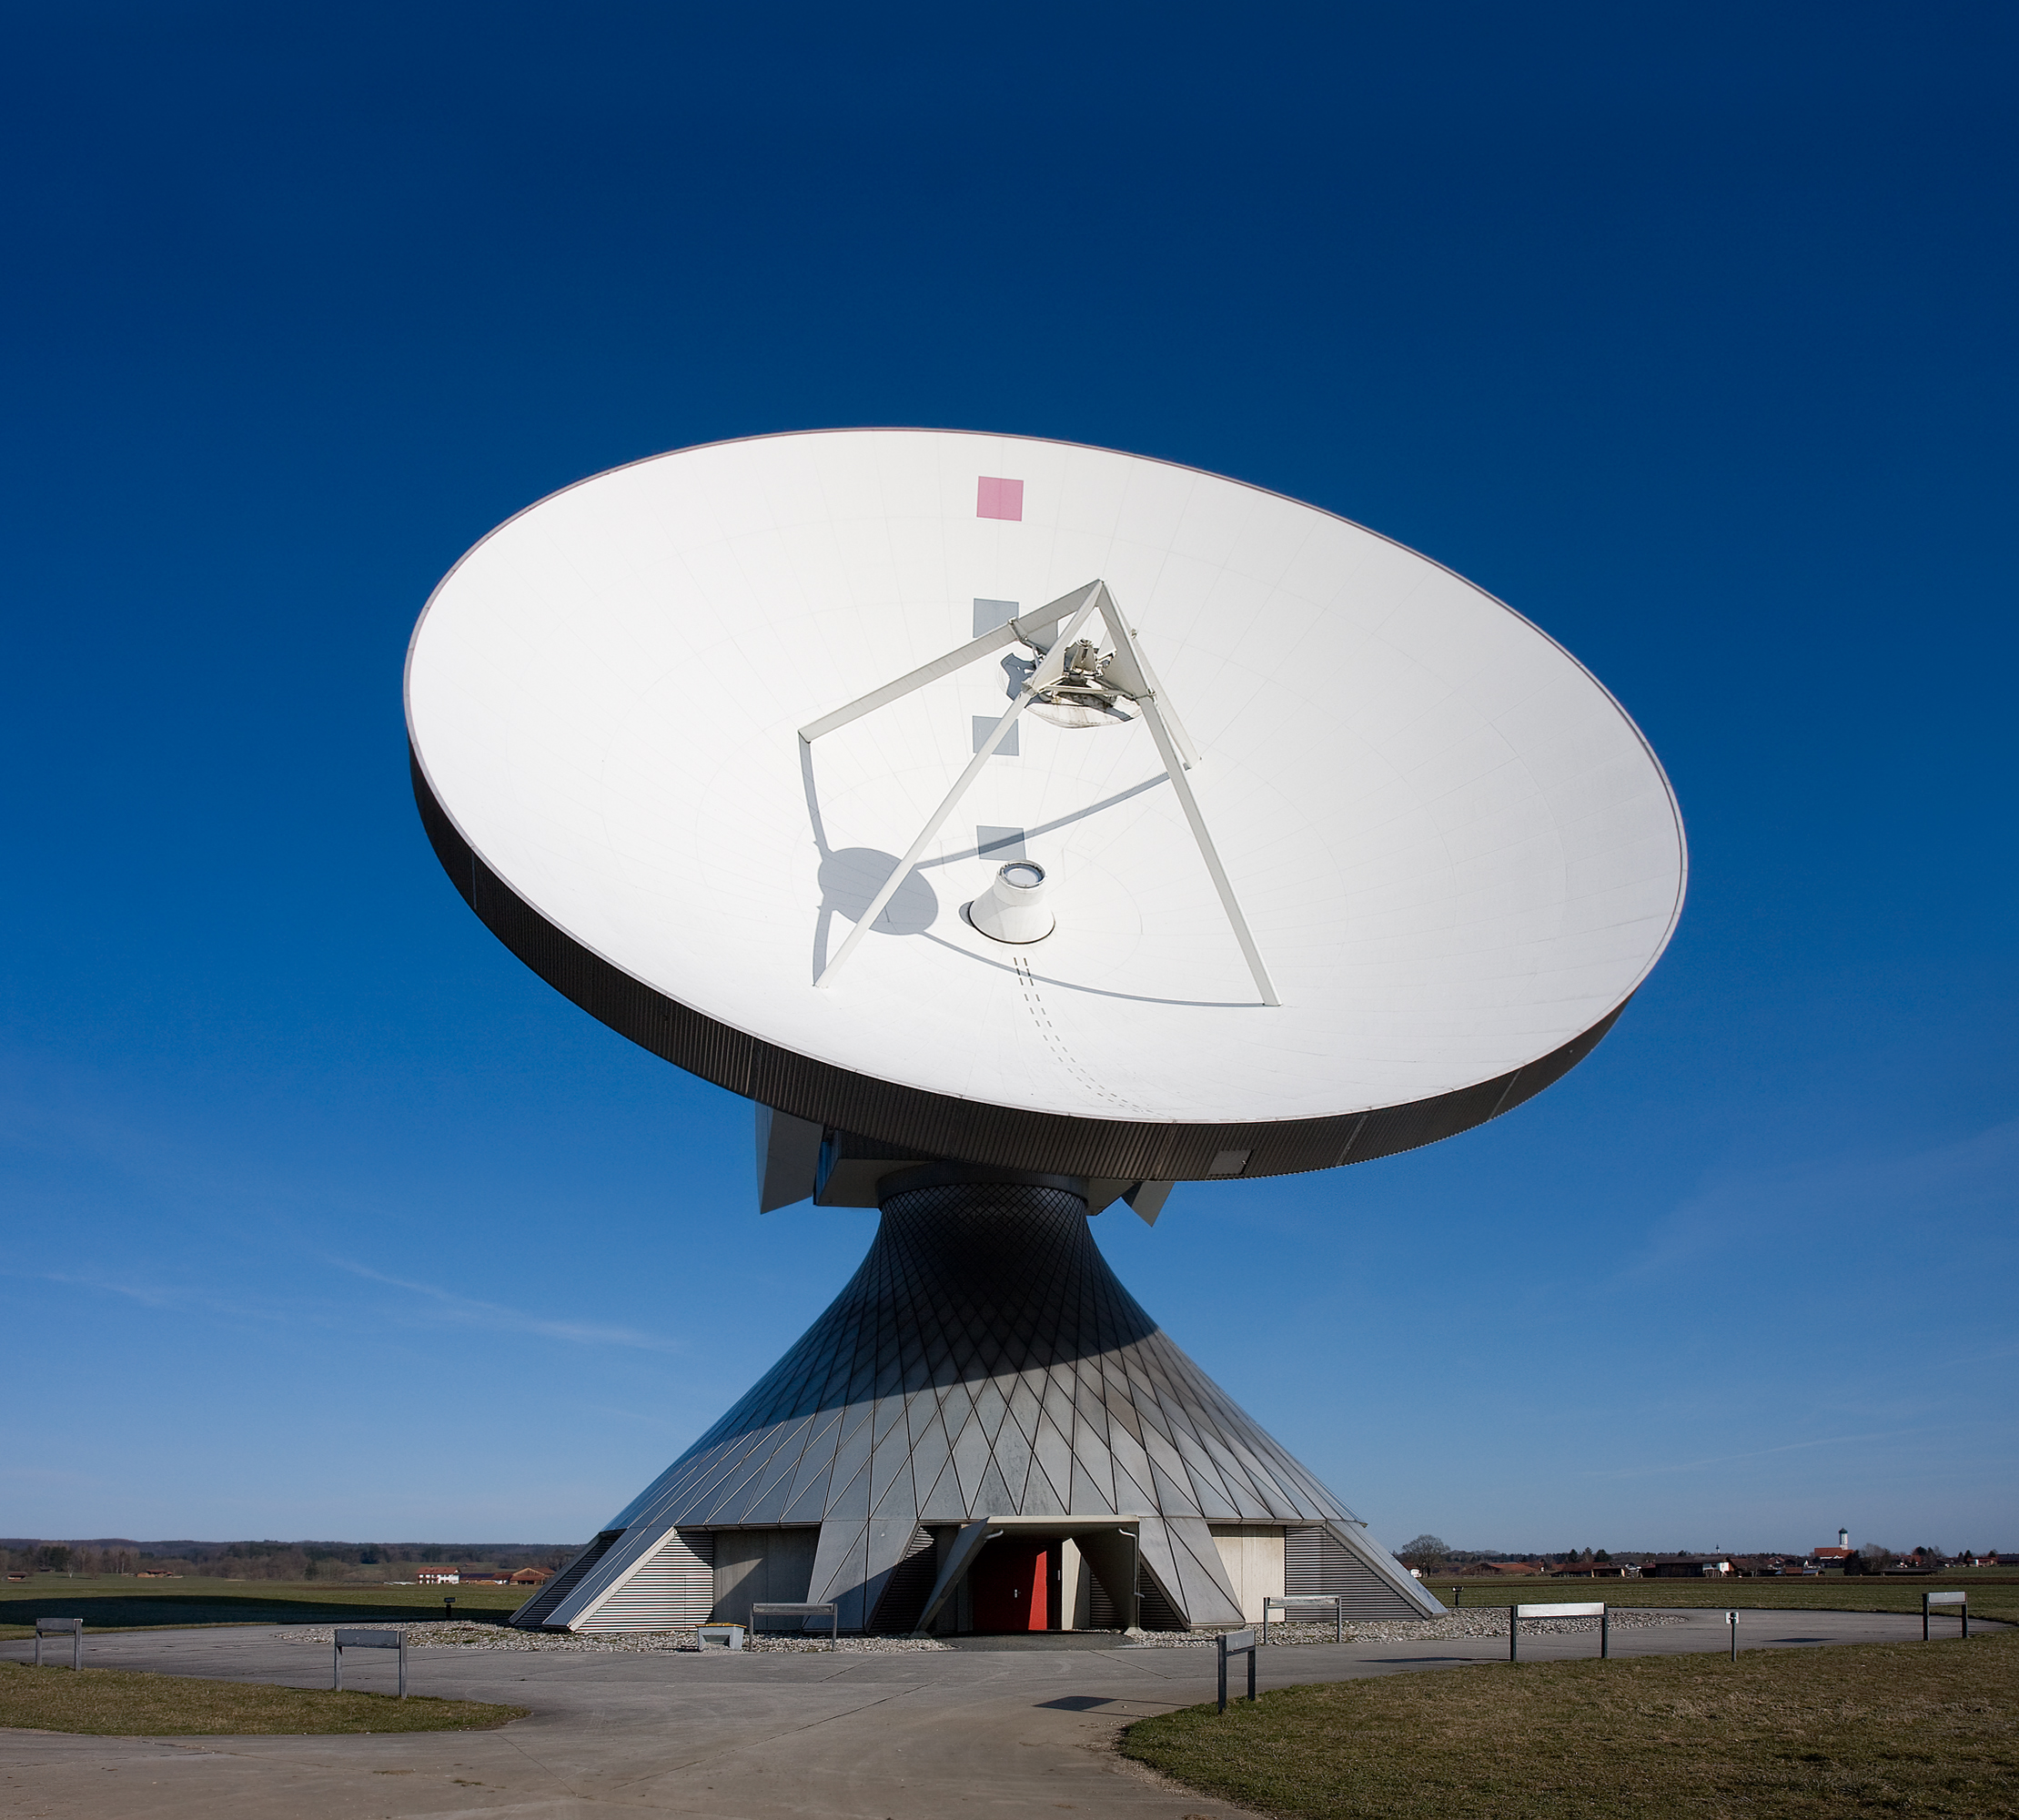
\includegraphics[scale=.1]{imagenes/antena.jpg}\\
Antena parabólica
}

\begin{wrapfigure}[12]{L}{8cm}
\psset{unit=1cm}
\begin{pspicture}(-0.8,0)(7,4)
\psline{->}(-0.8,.5)(7,.5)
\psline{->}(2,0                                                                                                                                                                                                                                                                                                                                                                                                                                                                                                                                                                                                                                                                                                                                                                                                                                                                                                                                                                                                                         
                                                                                                                                                                                                                                                                                                                                                                                                                                                                                                                                                                                                                                                  )(2,4)
\rput(6.8,.25){$x$}
\rput(1.8,3.8){$y$}
\psline[linestyle=dashed](-.7,.5)(5,4)
\psbezier(1,.5)(1,1.25)(3,3.7)(7,4)
\pscircle*(2.9,2.7){.1}
\psline(2,0.5)(2.9,2.7)
\psline{->}(2,0.5)(2.3,1.21)
\psline{->}(2.9,2.7)(7,2.7)
\psarc{->}(2,0.5){1}{0}{67.75}
\psarc{-}(2.9,2.7){0.7}{213}{247}
\rput(2.5,0.8){$\theta$}
\rput(3.2,2){$\alpha$}
\rput(0.2,0.7){$\phi$}
\psline{->}(3,2)(2.9,2)(2.6,2.5)
\psarc{-}(2.9,2.7){2}{0}{33}
\rput(4,2.9){$\beta$}
\end{pspicture}
\caption{Reflejo en un espejo curvo}
\end{wrapfigure}






 \noindent\textbf{Solución.} Sea $(x,y)$ el punto de incidencia. Apelando a la geometría elemental, $\phi=\beta$ y $\theta=\alpha+\phi=2\beta$. Como $\tan\theta=\frac{y}{x}$
  y como
  \[\begin{split} \tan\theta &=\tan 2\beta\\&=\frac{2\tan\beta}{1-\tan^2\beta},
    \end{split}
\]
deducimos que
\[\frac{y}{x}=\frac{2 dy/dx}{1-(dy/dx)^2}.\]
Despejando
\begin{equation}\label{eq:antena}
 (\pm\sqrt{x^2+y^2}+x)dx+ydy=0
\end{equation}
La expresión sugiere introducir coordenadas polares
\[x=r\cos\theta, \quad y=r\sen\theta.\]
Atendiendo a \eqref{eq:formas} tenemos:
\[dx=\cos\theta dr-r\sen\theta d\theta,\quad dy=\sen\theta dr+r\cos\theta d\theta.\]
Sustituyendo en \eqref{eq:antena}

\[\mp r^{2} \sin{\left (\theta \right )} d\theta + \left(\pm r \cos{\left (\theta \right )} + r\right) dr=0.\]
Notar que
\[\frac{N_{\theta}-M_r}{M}=-\frac{1}{r}\]
es independiente de $\theta$. Tenemos que $\mu(r)=r^{-1}$ es factor integrante. Multiplicando por $\mu$ llegamos a la ecuación exacta
\[\mp r\sen\theta d\theta+(\pm\cos\theta+ 1)dr=0.\]
Siguiendo las técnicas expuestas llegamos a la función potencial
\[\Phi(\theta,r)=\pm r\cos\theta +r.\]
Convirtiendo nuevamente a coordenadas cartesianas, encontramos que la solución general es
\[\pm x + \sqrt{x^2+y^2}=c.\]
Despejando
\[y^2=\mp 2xc+c^2=2c\left(\mp x+\frac{c}{2}\right)\]
Que es la familia de todas las parábolas con eje de simetría $x$  y con foco en $(0,0)$. 
El signo $\mp$ refleja el hecho que el espejo podría mirar hacia un lado u otro. 

\section{Ecuaciones Lineales}
\begin{definicion}[Ecuación lineal]{} Se llama \href{http://es.wikipedia.org/wiki/Ecuación_diferencial_lineal}{ecuación diferencial lineal}
a una ecuación que es lineal
respecto a   la/s variables
dependientes. La siguiente es la ecuación diferencial lineal general de primer orden
\begin{empheq}[box=\tcbhighmath]{equation}\label{eq:lineal}
 y'+p(x)y=q(x)
\end{empheq}

y la  de segundo orden
\begin{empheq}[box=\tcbhighmath]{equation}\label{eq:lineal_orden2}
 y''+p(x)y'+q(x)y=r(x).
\end{empheq}
 
Aquí $p,q$ y $r$ son funciones de $x$ usualmente definidas sobre un intervalo abierto de $\rr$.
\end{definicion}
La ecuación puede ser no lineal repecto a la variable independiente.

Es costumbre introducir los operadores  diferenciales $L_1[y]=y'+py$  y $ L_2[y]=y''+py'+qy$.
Para una ecuación lineal, los operadores $L_1$ y $L_2$ son lineales. Es decir, $L_1[y_1+y_2]=L_1[y_1]+L_1[y_2]$.


 Vamos a resolver la ecuación lineal de primer orden \eqref{eq:lineal}. Esto es sencillo pues la forma diferencial asociada
 \begin{equation}\label{eq:lineal2}dy+(p(x)y-q(x))dx=0
  \end{equation}
tiene un factor integrante que depende sólo de $x$. En efecto como $M=p(x)y-q(x)$ y $N=1$.
 \[\frac{\mu'}{\mu}=\frac{\partial M/\partial y-\partial N/\partial x}{N}=p(x).\]
 Entonces $\mu(x)=e^{\int pdx}$ es factor integrante. Luego si multiplicamos por $\mu$ en \eqref{eq:lineal2},  la expresión  es exacta.
 \[e^{\int pdx}dy+p(x)e^{\int pdx}ydx=q(x)e^{\int pdx}dx.\]
Podemos identificar rápidamente, sin necesidad de hacer cálculos, el correspondiente potencial.
 \[d\left(e^{\int pdx}y\right)=d\left(\int q(x)e^{\int p} dx \right).\]
Integrando
\[e^{\int pdx}y=\int e^{\int pdx}q(x)dx+C.
 \]
Entonces
\begin{empheq}[box=\tcbhighmath]{equation}\label{SolGenLin}
  y=e^{-\int pdx}\left\{\int e^{\int pdx}q(x)dx+C\right\} 
\end{empheq}


\begin{ejemplo}{}{} Resolver $y'+y/x=3x$.
 \end{ejemplo}


\noindent\textbf{Solución.} En la práctica, para evitar recordar fórmulas, se suele repetir el procedimiento que llevo a la fórmula \eqref{SolGenLin}, ahora, dado la cercanía
de su derivación, vamos a usarla  de manera directa. La solución general es

\[\begin{split} y(x)&=e^{-\int\frac{1}{x}dx}\left\{\int e^{\int\frac{1}{x}dx}3xdx+C\right\}\\
   &=\frac{1}{|x|}\left\{\int |x| 3xdx+C\right\}\\
   &=x^2+\frac{C}{|x|}\\
   &=x^2+\frac{C}{x}\\
  \end{split}
\]




\section{Reducción de orden}

Algunas ecuaciones de segundo orden
\begin{empheq}[box=\tcbhighmath]{equation}\label{Gen2Or}
 F(x,y,y',y'')=0
\end{empheq}

se pueden reducir a una de primer orden. Por ejemplo si $F$ no depende de $y$. Es decir la ecuación es
\begin{empheq}[box=\tcbhighmath]{equation}
 F(x,y',y'')=0
\end{empheq}



Aquí introducimos la nueva variable dependiente $\boxed{p=y'}$, que resuelve
\[F(x,p,p')=0.\]
Que es una ecuación de primer orden. Supuesto que la podemos resolver y encontrar una solución general para  $p$, tendremos
\begin{empheq}[box=\tcbhighmath]{equation}
 y=\int pdx+C
\end{empheq}


Es la solución general de la ecuación de segundo orden.


Si la ecuación general de segundo orden \eqref{Gen2Or} no depende de $x$, es decir tenemos
\boxed{F(y,y',y'')=0}
entonces nuevamente usaremos $\boxed{p=y'}$ como nueva variable depeniente
pero también  $\boxed{y}$ como nueva variable independiente. Como
\[y''=p'=\frac{dp}{dx}=\frac{dp}{dy}\frac{dy}{dx}=\frac{dp}{dy}p\]
La ecuación se reduce a la siguiente ecuación de primer orden
\begin{empheq}[box=\tcbhighmath]{equation}\label{RedOrdSinInd}
 F\left(y,p,\frac{dp}{dy}p\right)=0
\end{empheq}

% 


\section{Aplicaciones}


\subsection{Velocidad de escape}\label{pag:vel_esc}


\begin{mdframed}[style=MiEstilo]\relax%
 \textbf{Velocidad de escape.} Que velocidad hay que imprimirle a un proyectil que es lanzado verticalmente desde la superficie de la Tierra si nuestra pretensión
es que el proyectil se escape al infinito. La velocidad más chica con esta cualidad se llama
\href{http://es.wikipedia.org/wiki/Velocidad_de_escape}{velocidad de escape}.
\end{mdframed}


\begin{wrapfigure}[15]{R}{5cm}

\begin{pspicture}(0,0)(4,4.3)
\psset{unit=1cm}
\pscircle[linestyle=none,fillstyle=solid,fillcolor=color8](1.5,1.5){1.5}
\psline(1.5,1.5)(2,2.91)
\psline(1.5,1.5)(2.5,4.32)
\pscircle*(2.5,4.32){.1}
\rput(1.32,1.55){\rotatebox{70}{\psline[linewidth=.01](0,-.2)(0,.2)
\psline[linewidth=.01](0,0)(0.6,0)
\psline[linewidth=.01](0.95,0)(1.5,0)
\psline[linewidth=.01](1.5,-.2)(1.5,.2)
\psline[linewidth=.01](1.5,0)(2.1,0)
\psline[linewidth=.01](2.45,0)(3,0)
\psline[linewidth=.01](3,-.2)(3,.2)
}}
\rput(1.6,2.3){\rotatebox{70}{$R$}}
\rput(2.1,3.7){\rotatebox{70}{$x$}}
\rput(.7,1.8){$M$}
\rput(2.85,4.32){$m$}
\end{pspicture}
\caption{Velocidad de Escape}\label{fig:vel_esc}
\end{wrapfigure}

 \noindent\textbf{Solución.} Para resolver este problema hay que tomar en consideración la
\href{http://es.wikipedia.org/wiki/Ley_de_gravitación_universal}{Ley de gravitación universal}
de Newton. En la parte que nos interesa, esta Ley afirma
que el módulo de la fuerza de gravedad que se ejercen entre si dos cuerpos de masa $m_1$ y $m_2$ separados una distancia $r$ es proporcional al producto de las masas
e inversamente proporcional al cuadrado de las distancia que los separa. Vale decir
\[|F|=G\frac{m_1m_2}{r^2},\]
donde $G$ es la constante de proporcionalidad.
Cuando los cuerpos no son puntos masa, sino esferas de dendsidad uniforme la distancia de separación hay que medirla entre los centros de masa de los cuerpos.



Hay que aclarar que usando el 
\href{https://docs.google.com/file/d/0B80iJ0HgObRRWll6MlJFSjFNMGc/edit}{Principio conservación energía mecánica}\linebreak podemos resolver
el problema de una manera más simple. Incluso podemos ver que la suposición de que el tiro es vertical no es necesaria, es decir la velocidad de escape es la misma aunque
el tiro sea oblicuo. Discutiremos esa solución durante la clase. Lamentablemente,  esta solución no usa ecuaciones diferenciales.
Vamos a dar una solución, quizás un poco más complicada, pero que invoca las técnicas
discutidas.


Supondremos a la Tierra una esfera de radio $R$, masa $M$ y su centro de masa en el centro de la esfera.   Al proyectil lo supondremos un punto masa
con masa $m$ y su posición en el momento $t$, denotada $x=x(t)$, la mediremos sobre un eje vertical con origen en la
superficie de la Tierra.  Todo como está indicado en la figura \ref{fig:vel_esc}.
Luego la distancia Tierra-proyectil será igual a $R+x$ donde $x$ es la posición del proyectil. Utilizando la 
\href{http://es.wikipedia.org/wiki/Leyes_de_Newton\#Segunda_ley_de_Newton_o_ley_de_fuerza}{Segunda ley de Newton},
$F=ma$, obtenemos
\[mx''(t)=-\frac{GMm}{(R+x)^2}.\]
Es una ecuación de la forma
\[F(x,x',x'')=0.\]
Con variable dependiente $x$ e independiente $t$. Pero  $F$ no depende de $t$ y por consiguiente, como vimos, se puede convertir en una ecuación de primer orden
tomando como nuevas variables: 1) independiente $x$ 2) dependiente $v=x'$. En estas variables
\[\frac{d^2x}{dt^2}=\frac{dv}{dt}=\frac{dv}{dx}\frac{dx}{dt}=v\frac{dv}{dx}.\]
La ecuación se convierte en
\[v\frac{dv}{dx}=-\frac{GM}{(R+x)^2}\Longrightarrow vdv+\frac{GM}{(R+x)^2}dx=0.\]
Que es una ecuación en variables separables y también es exacta. Usaremos la técnica discutida para
ecuaciones exactas \marginpar{Siempre las ecuaciones en variables separables son exactas pues se escriben de la forma
\[{ \scriptscriptstyle M(x)dx+N(y)dy=0,}\]
por consiguiente tienen potencial
\[{ \scriptscriptstyle f=\int M(x)dx +\int N(y)dy}\]}, los que nos indica que la solución general se expresa de la siguiente forma
\begin{equation}\label{energia}
 \frac{v^2}{2}-\frac{GM}{(R+x)}=E=\text{cte}.
\end{equation}


La igualdad anterior es precisamente  consecuencia directa del \href{https://docs.google.com/file/d/0B80iJ0HgObRRWll6MlJFSjFNMGc/edit}{Principio conservación energía mecánica},
La hemos deducido como consecuencia de que la ecuación era exacta. 
Sea $v_0$ la velocidad inicial para $t=0$. 
Como $E$ es constante y $x=0$ en $t=0$ debemos tener
\begin{equation}\label{energia_cero}
 E=\frac{v_0^2}{2}-GM/R
\end{equation}
Como $v^2\geq 0$ y por \eqref{energia} y \eqref{energia_cero}.
\[-\frac{GM}{(R+x)}\leq\frac{v^2}{2}-\frac{GM}{(R+x)}=\frac{v_0}{2}-\frac{GM}{R}\]
Queremos encontrar $v_0$ tal que $x\to\infty$. Si tomamos
límite cuando $x\to\infty$ en la expresión anterior obtenemos
\[0\leq \frac{v_0^2}{2}-GM/R\]
De aquí deducimos que el valor mínimo de velocidad de escape es 
$\sqrt(2*GM/R)$.

\subsection{Curvas de persecución}

\begin{mdframed}[style=MiEstilo]\relax%
\textbf{Curvas de persecución.} Supongamos que un conejo se mueve sobre una
línea recta con rapidez uniforme $a$ y de un punto por fuera de la recta parte un perro que lo
persigue con rapidez uniforme $b$. Encontrar la trayectoria del perrro.
\end{mdframed}







\begin{figure}[h]
\begin{center}
\animategraphics[controls, scale=.4]{15}{pursuit/pursuit-}{0}{40}
 \caption{\small Persecución en un pentágono estrellado.
\href{https://www.sciencenews.org/article/art-pursuit-3}{Art of Pursuit},
Ivars Peterson
}
\end{center}
\end{figure}



\begin{wrapfigure}[15]{R}{5cm}



\scalebox{.6} % Change this value to rescale the drawing.
{
\begin{pspicture}(0,-4.51)(8.68,4.51)
\psline[linewidth=0.04cm,arrowsize=0.05291667cm 2.0,arrowlength=1.4,arrowinset=0.4]{->}(0.8,-4.49)(0.8,4.49)
\psline[linewidth=0.04cm,arrowsize=0.05291667cm 2.0,arrowlength=1.4,arrowinset=0.4]{->}(0.0,-3.49)(8.66,-3.53)
\psbezier[linewidth=0.04](2.52,2.11)(2.52,1.33)(3.44,-3.49)(7.34,-3.51)
\psline[linewidth=0.04cm,linestyle=dashed,dash=0.16cm 0.16cm](3.4,-0.77)(0.82,3.09)
\rput(1.9,3.12){$C=(0,at)$}
\rput(0.3,4){$y$}
\rput(8.66,-3.8){$x$}
\rput(2.2,-0.77){$P=(x,y)$}
\rput(7.34,-3.8){$(c,0)$}
\rput(5.4,-1.8){$s$}
\psdots[dotsize=0.12](3.36,-0.75)
\psdots[dotsize=0.124](3.34,-0.75)
\psdots[dotsize=0.154](3.34,-0.73)
\psbezier[linewidth=0.012](7.34,-3.13)(6.34,-3.15)(4.66,-1.79)(3.92,-0.45)
\psline[linewidth=0.0139999995cm](4.16,-0.31)(3.64,-0.63)
\psline[linewidth=0.0139999995cm](7.34,-2.85)(7.34,-3.39)
\psdots[dotsize=0.012](0.84,3.09)
\psdots[dotsize=0.012](0.84,3.09)
\psdots[dotsize=0.042](0.8,3.05)
\psdots[dotsize=0.103999995](0.82,3.05)
\psdots[dotsize=0.162](0.84,3.09)
\end{pspicture} 
}
\caption{Curva persecución}\label{fig:curva_per}
\end{wrapfigure}



Supongamos que el perro parte del punto $(c,0)$, el conejo de $(0,0 )$ y se mueve 
en línea recta en la dirección positiva  del eje $y$.
Vamos a suponer que el perro sigue la trayectoria donde
la tangente a su movimiento, en un momento dado, 
intersecta a la posición del conejo correspondiente a ese momento.


Pasado un tiempo $t$, el conejo estará en el punto $(0,at)$ y el perro en un punto de su trayectoria que forma un arco de
 longitud $s=bt$ hasta el punto $(c,0)$. Ese punto, donde está el perro, lo denotaremos $(x,y)$. Como hemos supuesto que la tangente a la trayectoria del perro en $(x,y)$ pasa
 por la posición del conejo $(0,at)$ se debe cumplir que
 \begin{equation}\label{eq:persec}\frac{dy}{dx}=\frac{y-at}{x}\Longrightarrow xy'-y=-at.\end{equation}
 En esta ecuación hay tres variables, $t$ , $x$ e $y$. No hemos definido cuales 
 son independiente y cuales depenientes.   Generalmente el tiempo $t$ se considera  
 variable  indepeniente, pero en la expresión de arriba aparece la derivada de $y$ 
 respecto a $x$.
 Claramente deberíamos eliminar una de las variables. Conviene eliminar $t$, dado que 
 al no aparecer en la derivación no tendremos que hacer un cambio de variables allí, 
 donde siempre es un poco más engorroso.   Por otra parte, la intuición del problema, 
 nos dice que  a cada $t$ corresponde uno, y sólo un, $x$\footnote{De lo contrario el 
 perro no se hubiera movido en la dirección horizontal entre dos momentos, lo que es absurdo}, lo que indica que $t$ es función de $x$ y por consiguiente es de esperar poder escribir la ecuación \eqref{eq:persec} en términos de $x$ e $y$.   Tener en cuenta que no es  razonable en matemática, como en la política,  pensar que lograremos tener un beneficio (menos variables) sin pagar algún precio, pues, como dice el dicho,
 ``Cuando la limosna es grande hasta el santo desconfía'' .
 En este caso, el costo que pagaremos
 es incrementar el orden de la ecuación.
 Como hemos dado algunas técnicas de  resolver ecuaciones de orden dos, quizás estemos en condiciones de pagar este precio.

Para eliminar $t$ de la ecuación \eqref{eq:persec}, derivamos $\eqref{eq:persec}$ respecto a $x$, para obtener
\[xy''=-a\frac{dt}{dx}.\]
Como $ds/dt=b$
\[\frac{dt}{dx}=\frac{dt}{ds}\frac{ds}{dx}=-\frac{\sqrt{1+y'(x)^2}}{b}.\]
Hemos usado la relación $s=\int_x^c\sqrt{1+y'^2}dx$.
 Entonces
 \begin{empheq}[box=\tcbhighmath]{equation}xy''=\frac{a\sqrt{1+y'(x)^2}}{b}.
   \end{empheq}


Que es una ecuación que no contiene $y$. De modo que usando $p=y'$ como variable dependiente reducimos el orden de la ecuación. Nos queda
\[\frac{dp}{\sqrt{1+p^2}}=\frac{a}{b}\frac{dx}{x}.\]
Que es una ecuación en variable separables. Tomando la integral definida entre $c$ y $x$, y considerando que si $x=c$ entonces $p=0$, tenemos
\[\ln\left(p+\sqrt{1+p^2}\right)=\ln\left( \frac{x}{c}\right)^{\tfrac{a}{b}}.\]
 Si despejamos $p$ conseguimos
 \begin{empheq}[box=\tcbhighmath]{equation}p=\frac{dy}{dx}=\frac{1}{2}\left[\left(\frac{x}{c}\right)^{a/b}-\left(\frac{c}{x}\right)^{a/b}\right]. 
 \end{empheq}

Para hallar $y$ hay que recordar que $y'=p$ e $y(1)=0$.

Usemos \texttt{SymPy} para completar este cálculo y hacer los gráficos. El siguiente código evalúa la integral, halla la constante de integración para que $y(1)=0$ y grafica.


Los resultados son:

\begin{tabular}{m{4cm} m{4cm} m{4cm}}
\begin{center}
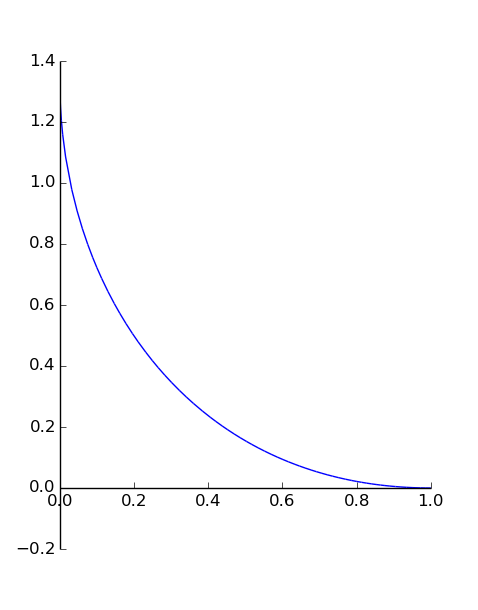
\includegraphics[scale=.3]{imagenes/perse_a_1_b_2.png}

$a<b$
\end{center}
&
\begin{center}
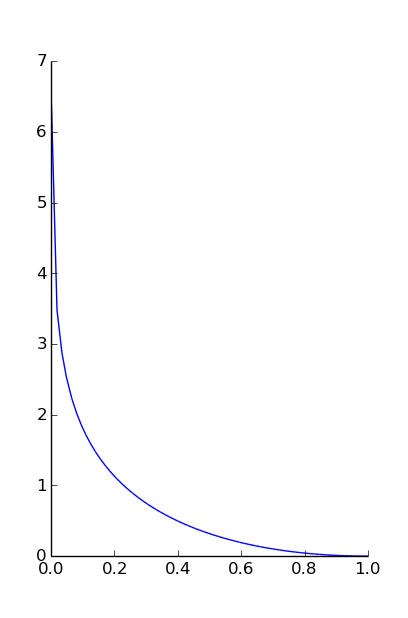
\includegraphics[scale=.3]{imagenes/perse_a_1_b_1.png}

$a=b$
\end{center}
&
\begin{center}
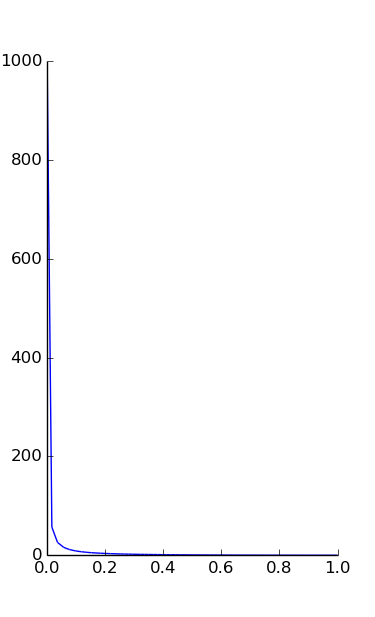
\includegraphics[scale=.3]{imagenes/perse_a_2_b_1.png}

$a>b$
\end{center}

\end{tabular}



Lo anterior constituye un ejemplo de lo que se conoce como\marginpar{
 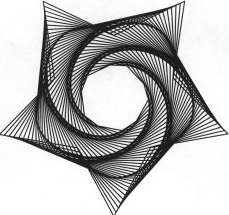
\includegraphics[scale=.4]{imagenes/persecucion2.jpg}\\
Persecución en un pentágono estrellado. Extraído de\\
\href{https://www.sciencenews.org/article/art-pursuit-3}{Art of Pursuit},
} \href{https://en.wikipedia.org/wiki/Pursuit_curve}{curva de persecución}. Este es un tema muy interesante que tiene varias generalizaciones, por ejemplo el \href{https://en.wikipedia.org/wiki/Mice_problem}{problema de los ratones} donde se colocan en cada vértice de un polígono ratones cada uno de los cuales persigue al vecino en sentido antihorario (u horario, da lo mismo). Se consiguen patrones geométricos myu bellos




\section{Oscilador armónico}\label{resortito}




Un \href{http://es.wikipedia.org/wiki/Oscilador_armónico}{oscilador armónico} es el más simple de los sistemas físicos vibratorios. Podemos definirlo como un sistema
elástico que obedece a la \href{http://es.wikipedia.org/wiki/Ley_de_Hooke}{Ley de elasticidad de Hooke}, en honor a su descubridor
\href{http://es.wikipedia.org/wiki/Robert_Hooke}{Robert Hooke (1635-1703)}.
\marginpar{
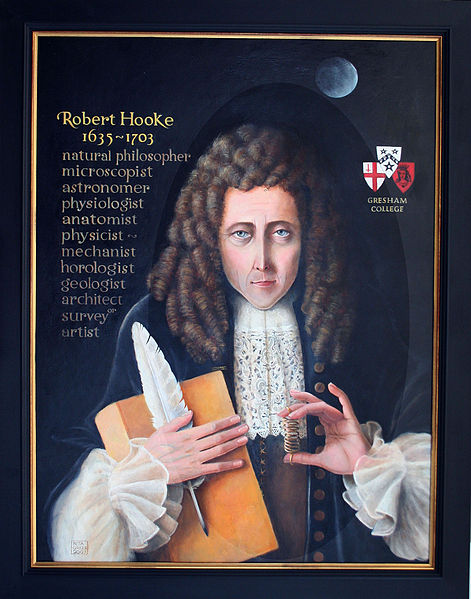
\includegraphics[scale=.15]{imagenes/Hooke.JPG}\\
Robert Hooke
}

Suele citarse al \href{http://es.wikipedia.org/wiki/Resorte}{resorte} como un ejemplo familiar de oscilador armónico. Esto debido a que, cuando las oscilaciones de un resorte son
pequeñas,  se satisface aproximadamente la Ley de elasticidad de  Hooke. Esta ley  afirma que la fuerza que ejerce un resorte sobre una masa $m$ conectada a él por uno
de sus extremos es proporcional en magnitud al desplazamiento
del resorte desde la posición de equilibrio. Además la fuerza de elasticidad actúa en sentido opuesto al desplazamiento.

\begin{figure}[h]
 \begin{center}
  \animategraphics[controls, scale=.4]{15}{resorte/resorte-}{0}{47}
 \caption{Resorte}\label{fig:resortito}
 \end{center}
 \end{figure}

 Supongamos que tenemos un resorte, en unos de sus extremos fijado en una pared y unido a una masa $m$ por el otro extremo. Supongamos que no actúa otra fuerza
 sobre la masa mas que la del resorte. Ver la animación de la figura \ref{fig:resortito}.  Pongamos un eje de coordenadas en la dirección del movimiento, con origen en la posición de equilibrio
 del resorte. Esta posición es el punto donde el resorte no ejerce fuerza. Supongamos que la dirección positiva es la dirección donde el resorte se expande. Denotemos
 por $x(t)$ la posición de la masa en el momento $t$.    Entonces según la Segunda Ley de Newton y la Ley de Elasticidad de Hooke, tenemos que

 \begin{empheq}[box=\tcbhighmath]{equation}mx''(t)=-kx(t).\label{eq:resorte}
 \end{empheq}


La constante de proporcionalidad $k$ se llama \href{http://es.wikipedia.org/wiki/Rigidez}{constante elástica}. La ecuación \eqref{eq:resorte} se denomina la
ecuación del oscilador armónico o ecuación del resorte.

La ecuación del oscilador armónico se escribe $0=f(t,x,x',x'')$, donde \linebreak $f(t,x,y,z)=kx+mz$ es independiente de $t$. Podemos intentar usar $x$ como variable
independiente y $z=x'$ como dependiente. Como vimos  $x''(t)=dz/dt=dz/dx z$. Así la ecuación queda
\[\begin{split}
   m\frac{dz}{dx}z=-kx &\Longrightarrow mzdz=-kxdx\Longrightarrow m\frac{z^2}{2}=-k\frac{x^2}{2}+C_1\\
   &\Longrightarrow z=\pm\sqrt{-\frac{k}{m}x^2+C_1}\\
   &\Longrightarrow x'(t)=\pm\sqrt{-\frac{k}{m}x^2+C_1}.\\
  \end{split}
\]
Debe ser $C_1\geq 0$ de lo contrario el dominio de la función sería vacío. Nos queda una nueva ecuación para $x'$.
Esta ecuación es en variables separables
\[ \frac{dx}{\sqrt{-\frac{k}{m}x^2+C_1}}=dt.
\]
 Integrando
\[\begin{split}
   t+C_2
   &=\int \frac{dx}{\sqrt{-\frac{k}{m}x^2+C_1}}\\
   &= \sqrt{\frac{1}{C_1}} \int \frac{dx}{\sqrt{-\frac{k}{C_1m}x^2+1}} \\
   &= \sqrt{\frac{m}{k}} \int \frac{du}{\sqrt{1-u^2}}\quad \left(\text{haciendo } u=\sqrt{\frac{k}{C_1m}}x\right)\\
   &=\sqrt{\frac{m}{k}}\arcsen u.
  \end{split}
\]
Entonces
\[\begin{split}
    x=\frac{C_1m}{k}u &=\frac{C_1m}{k}\sen \left(\sqrt{\frac{k}{m}}(t+C_2)\right)\\
    &=\boxed{C_3\sen \sqrt{\frac{k}{m}}t+C_4\cos \sqrt{\frac{k}{m}}t}.
  \end{split}
 \]
Que es la solución general\footnote{Esta afirmación se justificará en el capítulo 3}  de la ecuación del oscilador armónico. Como vemos el movimiento es oscilatorio con frecuencia
\[\boxed{f=\sqrt{\frac{k}{m}} }.\]
En particular, no importan las condiciones iniciales, la frecuencia es siempre la misma.






\section{EDP, método características}

Saber resolver ecuaciones ordinarias de primer orden nos permite resolver algunas ecuaciones en derivadas parciales de primer orden.  Vamos a exponer este punto a través del \href{https://en.wikipedia.org/wiki/Method_of_characteristics}{método de características}.

Para tener un problema bien planteado con  ecuaciones en derivadas parciales no es suficiente conocer el valor de la función en un punto (como en una EDO de primer orden). Una condición típica extra, para lograr este propósito,  es consignar el valor de la función a lo largo de una curva, que por simplicidad asumiremos que es una recta .

\begin{ejemplo}{} Resolver
\begin{equation}\label{eq:EDP_gral_1orden}
  \left.\begin{array}{l}
  a(x,y)u_x+b(x,y)u_y=c(x,y,u)\\
  u(x,0)=f(x)\\
\end{array}\right\}
\end{equation}
Aquí $x,y$ son variables independientes y $u$ dependiente. La primera línea es la ecuación diferencial, que incluye derivadas parciales de la incognita y la segunda línea podemos denominarla condición inicial (pensando que la variable $y$ representa tiempo).
\end{ejemplo}

El método de características consiste en encotrar $u$ a lo largo de las soluciones de la EDO

\begin{empheq}[box=\tcbhighmath]{equation}\frac{dy}{dx}=\frac{b(x,y)}{a(x,y)}\label{eq:ecua_caract}
\end{empheq}
Una solución de esta ecuación es normalmente una curva en el plano  $x,y$. La idea es que las soluciones de \eqref{eq:ecua_caract} forman un flia uniparamétrica
 de curvas que llena una parte $\Omega$ del plano $x,y$.  Así terminamos conociendo el valor de $u$ sobre este conjunto $\Omega$. Para que \eqref{eq:ecua_caract} tenga sentido debemos tener $a\neq 0$. De todas formas si $a=0$ podemos invertir los roles de $x$ e $y$.

Supongamos $y(x)$ solución de \eqref{eq:ecua_caract}, entonces pongamos por abuso de notación $u(x)=u(x,y(x))$. Se tiene que

\begin{empheq}[box=\tcbhighmath]{equation}\frac{du}{dx}=u_x+u_yy'=u_x+u_y\frac{b}{a}=\frac{c(x,y(x),u(x))}{a(x,y)}\label{eq:ecua_caract2}
 \end{empheq}

Que es otra ecuación ordinaria. Podemos escribir  \eqref{eq:ecua_caract} y \eqref{eq:ecua_caract2} en una ecuación más simétrica
\begin{empheq}[box=\tcbhighmath]{equation}\frac{du}{c}=\frac{dx}{a}=\frac{dy}{b}\label{eq:caract}
 \end{empheq}


Estas ecuaciones se llaman \emph{ecuaciones características}. Las soluciones de estas ecuaciones son un familia de curvas que suele llenar un conjunto abierto de  $\mathbb{R}^3$.  La gráfica de la solución se obtiene eligiendo entre estas curvas las que pasan por los puntos de la gráfica de $u$ especificados en la condición inicial, es decir $(x,0,f(x))$. Esto, en los casos favorables, forma una superficie que es la gráfica de la solución. La proyección de estas curvas en el plano $x,y$ se denominan \emph{caracterísitcas}. Son la familia de soluciones de $y'=b/a$.


\begin{ejemplo}{} Resolver
\begin{equation}\label{eq:EDP_gral_1orden}
  \left.\begin{array}{l}
  u_x+u_y=yu\\
  u(x,0)=f(x)\\
\end{array}\right\}
\end{equation}
\end{ejemplo}
En este caso
\[\frac{dy}{dx}=\frac{b}{a}\Rightarrow y'=1\Rightarrow y(x)=x+\mu,\quad\mu=\hbox{cte}.\]
Entonces
\[\frac{du}{dx}=\frac{c}{a}\Rightarrow u'=yu=(x+\mu)u\Rightarrow \ln|u|=\frac{x^2}{2}+\mu x+C(\mu).\]
Notar que la nueva constante de integración $C(\mu)$ debe depender de la primera $\mu$. Entonces
\[u=\pm e^{\frac{x^2}{2}}e^{(y-x)x}e^{C(y-x)}.\]
Ahora
\[u(x,0)=f(x)\Rightarrow f(x)=\pm e^{\frac{x^2}{2}}e^{-x^2}e^{C(-x)}\Rightarrow C(\mu)=\frac{\mu^2}{2}+\ln|f(-\mu)|.\]
Entonces
\[u(x,y)=\pm e^{\frac{x^2}{2}}e^{(y-x)x}e^{\frac{(y-x)^2}{2}+\ln|f(x-y)|        }
=e^{\frac{y^2}{2}}f(x-y).\]


\begin{subappendices}

\section{La braquistócrona}


\begin{mdframed}[style=MiEstilo]\relax% 
 Dados dos puntos $A$ y $B$ en las proximidades de la superficie terrestre, uno mas abajo respecto al suelo que el otro,
queremos diseñar el tobogán óptimo entre los dos,
esto es el tobogán que nos lleve de $A$ hasta $B$ en el menor tiempo. La curva solución a este problema se llama curva
\href{http://es.wikipedia.org/wiki/Curva_braquistócrona}{braquistócrona} (braquistos - el más corto, cronos - tiempo).
\end{mdframed}


\begin{center}
\animategraphics[controls,scale=.5]{15}{braquis/braquis-}{0}{105}
\end{center}


 Este problema fue resuelto por primera vez por Johann Bernoulli y es unos de los problemas precursores de la rama de las matemáticas que se denomina
\href{http://es.wikipedia.org/wiki/Cálculo_variacional}{cálculo de
variaciones}. Vamos a dar la solución del problema encontrada por  \marginpar{
    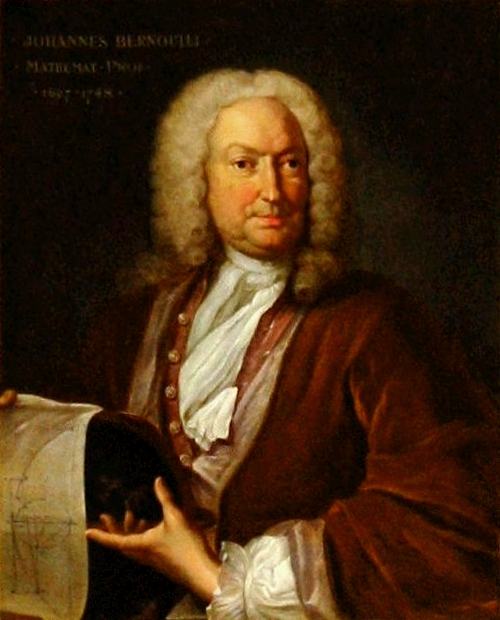
\includegraphics[scale=.2]{imagenes/Bernoulli.jpg}\\
    Johann Bernoulli (1667-1748)
}Johann Bernoulli que es muy elegante y está basada en un resultado de óptica llamado
 el \href{http://es.wikipedia.org/wiki/Principio_de_Fermat}{Principio de Mínimo Tiempo} de \href{http://es.wikipedia.org/wiki/Fermat}{Fermat}\marginpar{
    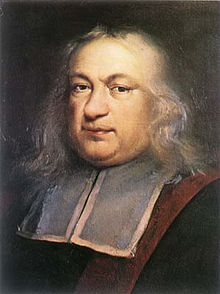
\includegraphics[scale=.3]{imagenes/Fermat.jpg}\\
    Pierre de Fermat (1601-1665)
}.

\begin{mdframed}[style=MiEstilo]\relax%
\href{http://es.wikipedia.org/wiki/Principio_de_Fermat}{\textbf {Principio de Mínimo Tiempo}} \textbf{de} \href{http://es.wikipedia.org/wiki/Fermat}{\textbf{Fermat}}
 La luz sigue para ir de un punto a otro el recorrido que minimiza el tiempo.
\end{mdframed}


 La primera impresión   es que ese reccorrido debería ser la línea recta. Si embargo esto no es así debido a que la velocidad de la luz cambia
de acuerdo al \href{http://es.wikipedia.org/wiki/Velocidad_de_la_luz_en_un_medio_material}{medio que atraviesa} .
La velocidad de la luz en el vacío es 299.792,458km/h y en el diamante 124.034,943 km/h. La velocidad de la luz cambia no sólo con la sustancia sino con sus cualidades,
como la densidad.

 Si la luz se mueve dentro de un medio homogéneo, el camino que sigue es la línea recta. Esto ya no es más así cuando la luz cambia de medio de propagación. Por ejemplo
cuando pasa del aire al vidrio.

\begin{wrapfigure}[12]{R}{5cm}

\begin{pspicture}(0,0)(5,4)
\psset{unit=1cm}
\psframe[linestyle=none,fillstyle=solid,fillcolor=color8](0,.3)(5,2)
\psline(0,2)(5,2)
\psline(0.5,2)(0.5,4)
\psline(0.5,3.7)(3.5,2)(4.7,0.3)
\psline(4.7,0)(4.7,2)
\psline[linestyle=dashed](3.5,0)(3.5,4)
\rput(3.75,1.3){$\alpha_2$}
\psarc{-}(3.5,2){1}{270}{306}
\rput(3.3,2.3){$\alpha_1$}
\psarc{-}(3.5,2){0.7}{90}{150}
\rput(1.1,3.8){$(a,0)$}
\rput(4.3,0){$(c,b)$}
\rput(3.3,1.8){$x$}
\pscircle*(0.5,3.7){.1}
\pscircle*(4.7,0.3){.1}

\end{pspicture}
\caption{Refracción de la luz}
\end{wrapfigure}
 Supongamos que la luz une los puntos $A$ y $B$ del plano y en el camino atravieza de un medio a otro, siendo la velocidad
 de la luz en cada uno de ellos $v_1$ y $v_2$.  Supongamos que $A=(a,0)$ y $B=(c,b)$ y el eje $x$ es la frontera entre los medios.

Como sabemos que mientras se mueva en un medio homogéneo la luz sigue en línea recta,
el tiempo que emplea la luz para ir $A$ a $B$ es
 \[t=\frac{\sqrt{a^{2} + x^{2}}}{v_{1}} + \frac{\sqrt{{\left(c - x\right)}^{2} + b^{2}}}{v_{2}}\]
Para determinar la trayectoria es suficiente encontrar $x$, el punto donde la luz choca con la interfaz entre los medios.
El principio de Fermat afirma que el tiempo es mínimo de modo que hallaremos un punto crítico de $t$ respecto a $x$.
\[ \frac{dt}{dx}=-\frac{c - x}{\sqrt{{\left(c - x\right)}^{2} + b^{2}} v_{2}} +
\frac{x}{\sqrt{a^{2} + x^{2}} v_{1}}=\frac{\sen\alpha_1}{v_1}-\frac{\sen\alpha_2}{v_2} \]
Deducimos que en un punto crítico
\begin{empheq}[box=\tcbhighmath]{equation}\frac{\sen\alpha_1}{v_1}=\frac{\sen\alpha_2}{v_2}\label{eq:ley_snell1}
\end{empheq}

que se denomina \href{http://es.wikipedia.org/wiki/Ley_de_Snell}{Ley de Snell}. El punto crítico es mínimo pues $\left.\frac{dt}{dx}\right|_{x=0}=-\tfrac{c}{bv_2}<0$ y
$\left.\frac{dt}{dx}\right|_{x=c}=\tfrac{c}{\sqrt{c^2+a^2}v_1}>0$.

 A la razón entre la velocidad de la luz dentro de un determinado medio y la velocidad de la luz en el vacio se lo denomina
\href{http://es.wikipedia.org/wiki/Índice_de_refracción}{índice de refracción} y se lo denota con la letra $n$. La Ley de Snell se la suele escribir
\[\boxed{n_1\sen\alpha_1=n_2\sen\alpha_2 }.\]
Que pasa si la luz atraviesa un medio que va cambiando de manera continua de índice de refracción. Por ejemplo, el índice de refracción en la atmósfera
va cambiando de manera continua con la altitud respecto a la superficie terrestre, ya que la densidad del aire va cambiando con la altitud. La Ley de
Snell en este caso es
\[\boxed{\frac{\sen\alpha}{v}=\text{cte}}\]
Aquí el ángulo $\alpha$ y la velocidad $v$ cambian respecto a alguna variable/s real/es, por ejemplo la altitud.


¿Que tienen en común el recorrido de la luz y la braquistócrona? Bernoulli se dió cuenta que la situación en los dos casos es la misma, ya que en los dos casos
se trata de minimizar el tiempo del recorrido. De modo que la braquistócrona también tiene que satisfacer la Ley de Snell.
 Ahora supongamos un sistema de coordenadas con origen en el punto $A$, inicial del recorrido.  Además supongamos que el movil  parte
del reposo. Con estas suposiciones $x(t_0)=0$ y $v(t_0)=0$. Por la conservación de la energía
\[\frac{m}{2}|v(t)|^2=-mgy(t)=mg|y(t)|.\]
 Así por la ley de Snell
\[\frac{\sen\alpha}{|v(t)|}=\frac{\sen\alpha}{\sqrt{2g|y|}}=c=\text{ cte}.\]
En \eqref{cos_alpha} habíamos expresado el $\cos\alpha$ (en realidad del ángulo opuesto por el vértice, pero es igual) mediante la derivada. Luego
\[\sen\alpha=\sqrt{1-\cos^2\alpha}=\frac{1}{\sqrt{1+y'(x)^2}}.\]
Entonces tenemos
\[\sqrt{2g|y|}\sqrt{1+y'(x)^2}=c=\hbox{ cte}\]
Despejando llegamos a la ecuación diferencial
\[\boxed{\sqrt{\frac{y}{c-y}}y'=1}.\]
Es una ecuación con variables separables. La constante $c$ no tiene el mismo valor que en la ecuación anterior.

La solución se obtiene resolviendo la integral
\[x=\int dx=\int \sqrt{\frac{y}{c-y}}dy.\]
lo que no es tan sencillo. Hacemos el cambio de variables
\[\sqrt{\frac{y}{c-y}}=\tan\phi\Longrightarrow y=c\sen^2\phi\Longrightarrow dy=2c\sen\phi\cos\phi d\phi.\]
Luego
\[x=2c\int\sen^2\phi d\phi=\frac{c}{2}\left(2\phi-\sen 2\phi\right)+C_1.\]
Como tiene que pasar por $x=0$ e $y=0$ debe ser $C_1=0$.  Tenemos que
 \[\left\{\begin{array}{l l l}
	      y&=c\sen^2 \phi&=\frac{c}{2}(1-\cos2\phi)\\
	      x&=\frac{c}{2}(2\phi-\sen2\phi)\ &\\
          \end{array}\right.
\]
Conviene llamar $2\phi=\theta$ y $a=c/2$
 \[\left\{\begin{array}{l l }
	      y&= a(1-\cos\theta)\\
	      x&=a(\theta-\sen\theta)\
          \end{array}\right.
\]
Que son la ecuaciones paramétricas de una curva conocida con el nombre de \href{http://es.wikipedia.org/wiki/Cicloide}{cicloide}. Podemos usar \texttt{SymPy} para graficar esta curva
\begin{pyverbatim}
theta=symbols('theta')
from sympy.plotting import *
plot_parametric(theta-sin(theta),1-cos(theta),(theta,0,10*pi))
\end{pyverbatim}

\begin{figure}[h]
\begin{center}
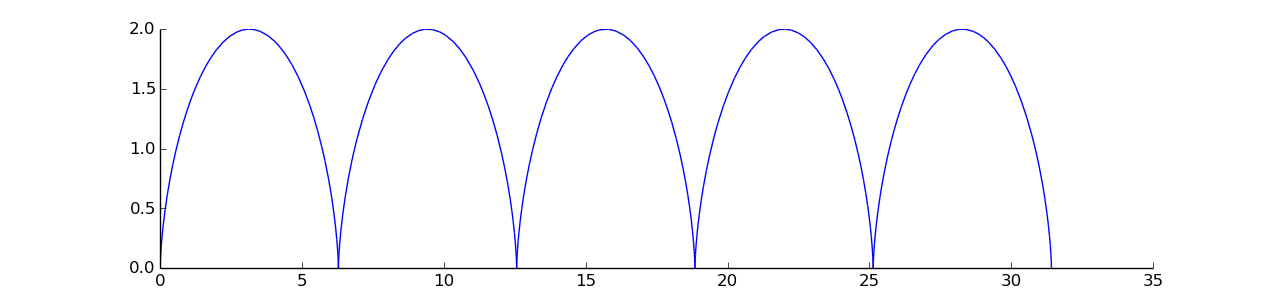
\includegraphics[scale=.3]{imagenes/cicloide.png}
\end{center}\caption{Cicloide}\label{fig:cicloide}
\end{figure}


\begin{figure}[h]
\begin{center}
\animategraphics[controls,scale=.5]{15}{cicloide/cicloide-}{0}{31}
\end{center}\caption{Cicloide}\label{fig:cicloide}
\end{figure}


Si in tentamos resolver las ecuaciones con \texttt{SymPy} el resultado no es muy alentador.

\begin{pyverbatim}
x,c=symbols('x,c')
y=Function('y')(x)
MiEcua=Eq(y.diff(x),sqrt((c-y)/y))
f=dsolve(MiEcua,y,hint='separable')
\end{pyverbatim}

\textbf{Resultado:}
\[
 \begin{cases} - i \sqrt{c} \sqrt{-1 + \frac{1}{c} y{\left (x \right )}} \sqrt{y{\left (x \right )}} - i c \operatorname{acosh}{\left (\frac{1}{\sqrt{c}} \sqrt{y{\left (x \right )}} \right )} & \text{for}\: \left\lvert{\frac{1}{c} y{\left (x \right )}}\right\rvert > 1 \\ \- \frac{\sqrt{c} \sqrt{y{\left (x \right )}}}{\sqrt{1 - \frac{1}{c} y{\left (x \right )}}} + c \operatorname{asin}{\left (\frac{1}{\sqrt{c}} \sqrt{y{\left (x \right )}} \right )} + \frac{y^{\frac{3}{2}}{\left (x \right )}}{\sqrt{c} \sqrt{1 - \frac{1}{c} y{\left (x \right )}}} & \text{otherwise} \end{cases} = C_{1} + x
\]



\section{La tautócrona}







  Vamos a ver otra propiedad notable de la ciclode. Supongamos que dejamos caer el cuerpo del reposo desde un punto intermedio, digamos en $(x_0,y_0)$. Sea  $\theta_0$
 el valor del paŕámetro $\theta$ correpondiente a este punto. ¿Cuánto tardara en llegar el cuerpo al punto mínimo de la curva que ocurre cuando $\theta=\pi$? 
% \begin{center}
% \animategraphics[controls,scale=.5]{15}{tautocrona/tauto-}{0}{79}
% \end{center}


  
  

 Tenemos
\[
 \left\{ \begin{array}{l l}
 \frac{dx}{d\theta}&=a(1-\cos\theta)\\
 \frac{dy}{d\theta}&=a\sen\theta 
 \end{array}\right.
\]
% 
Como el cuerpo ahora no parte de $(0,0)$ tendremos
\[|v|=\sqrt{2g(y_0-y)}.\]


  
Por \eqref{2ley} $ds/dt=|v|$. Si llamamos $T$ al tiempo que demanda en llegar a $\theta=\pi$, y llamamos  $s_0$ y $s_1$ a los arcos correspondientes al punto inicial
y final.  Tenemos
 \[T=\int_0^Tdt=\int_{s_0}^{s_1}\frac{dt}{ds}ds=\int_{s_0}^{s_1}\frac{1}{\sqrt{2g(y_0-y)}}ds.\]
Cambiando la variable de integración a $\theta$. Como 
\[
 \frac{ds}{d\theta}=\sqrt{\left(\frac{dx}{d\theta}\right)^2+\left(\frac{dy}{d\theta}\right)^2}=\sqrt{2}a\sqrt{1-cos\theta}.
\]
 Tenemos
\[T=\sqrt{\frac{a}{g}}\int_{\theta_0}^{\pi}\frac{\sqrt{1-\cos\theta}}{\cos\theta_0-\cos\theta}d\theta=
\sqrt{\frac{a}{g}}\int_{\theta_0}^{\pi}\frac{\sen\frac{\theta}{2}}{\cos^2\frac{\theta_0}{2}-\cos^2\frac{\theta}{2}}d\theta.
\]
Ahora hacemos la sustitución
\[u=\frac{\cos\frac{\theta}{2}}{\cos\frac{\theta_0}{2}}\Longrightarrow du=-\frac{\sen\frac{\theta}{2}}{2\cos\frac{\theta_0}{2}}d\theta.\]
Vemos que
\[
 T=2\sqrt{\frac{a}{g}}\int_0^1\frac{1}{\sqrt{1-u^2}}du.
\]
Que es una expresión independiente de $\theta_0$. En consecuencia el tiempo $T$ que demanda  el cuerpo para llegar $\theta=\pi$ es siempre el mismo no importa
desde donde se deje caer.

\begin{figure}[h]
\begin{center}
\animategraphics[controls,scale=.5]{15}{tautocrona/tauto-}{0}{79}
\end{center}\caption{Tautócrona}\label{fig:tautocrona}
\end{figure}

\section{Solución al problema del espejo con Sympy}
En este apéndice resolvemos el problema usando formas diferenciales
El submódulo diffgeom de Sympy implementa formas diferenciales. Del
sub-submodulo sympy.diffgeom.rn  importamos el objeto R2. 
Para comprender el funcionamiento del código remitimos a la 
\href{http://docs.sympy.org/latest/modules/diffgeom.html}{documentación de Sympy}.


\begin{pyblock}
from sympy import *
from sympy.diffgeom.rn import R2
eq=(-sqrt(R2.x**2+R2.y**2)+R2.x)*R2.dx+R2.y*R2.dy
M=eq.rcall(R2.e_theta)
N=eq.rcall(R2.e_r)
x,y,theta=symbols('x,y,theta')
r=symbols('r',positive=True)
subst={R2.x:r*cos(theta),R2.y:r*sin(theta),R2.theta:theta,R2.r:r}
M=M.subs(subst).simplify()
N=N.subs(subst).simplify()
mu=(N.diff(theta)-M.diff(r))/M
FactInt=exp(Integral(mu,r).doit())
phi=(M/r).integrate(theta)
g=Function('g')(r)
phi=phi+g
dsolve(phi.diff(r)-N/r,g)
phi=(M/r).integrate(theta)+r
phi
\end{pyblock}


$\py{latex(phi)}$

\end{subappendices}

  \bibliographystyle{apalike-url}
  \bibliography{diferenciales_ecuaciones,diferenciales_ecuaciones_sim}
%\end{document}
